%; whizzy chapter
% -initex iniptex -latex platex -format platex -bibtex jbibtex -fmt fmt
% $B0J>e(B whizzytex $B$r;HMQ$9$k>l9g$N@_Dj!#(B


%     Tokyo Debian Meeting resources
%     Copyright (C) 2009 Junichi Uekawa

%     This program is free software; you can redistribute it and/or modify
%     it under the terms of the GNU General Public License as published by
%     the Free Software Foundation; either version 2 of the License, or
%     (at your option) any later version.

%     This program is distributed in the hope that it will be useful,
%     but WITHOUT ANY WARRANTY; without even the implied warranty of
%     MERCHANTABILITY or FITNESS FOR A PARTICULAR PURPOSE.  See the
%     GNU General Public License for more details.

%     You should have received a copy of the GNU General Public License
%     along with this program; if not, write to the Free Software
%     Foundation, Inc., 51 Franklin St, Fifth Floor, Boston, MA  02110-1301 USA

%  preview (shell-command (concat "evince " (replace-regexp-in-string "tex$" "pdf"(buffer-file-name)) "&"))
% $B2hA|%U%!%$%k$r=hM}$9$k$?$a$K$O(Bebb$B$rMxMQ$7$F(Bboundingbox$B$r:n@.!#(B
%(shell-command "cd image200912; ebb *.png")

%%$B$3$3$+$i%X%C%@3+;O!#(B

\documentclass[mingoth,a4paper]{jsarticle}
\usepackage{monthlyreport}
\usepackage{wrapfig}

% $BF|IU$rDj5A$9$k!"Kh7nJQ$o$j$^$9!#(B
\newcommand{\debmtgyear}{2009}
\newcommand{\debmtgmonth}{12}
\newcommand{\debmtgdate}{12}
\newcommand{\debmtgnumber}{59}

\begin{document}

\begin{titlepage}
\thispagestyle{empty}

% $B%?%$%H%k%Z!<%8(B:$BJT=8I,MW$JItJ,$O:G=i$N%^%/%m$KHt$P$9$3$H(B

\vspace*{-2cm}
$BBh(B\debmtgnumber{}$B2s(B $BEl5~%(%j%"(B Debian $BJY6/2q;qNA(B

\hspace*{-2.4cm}
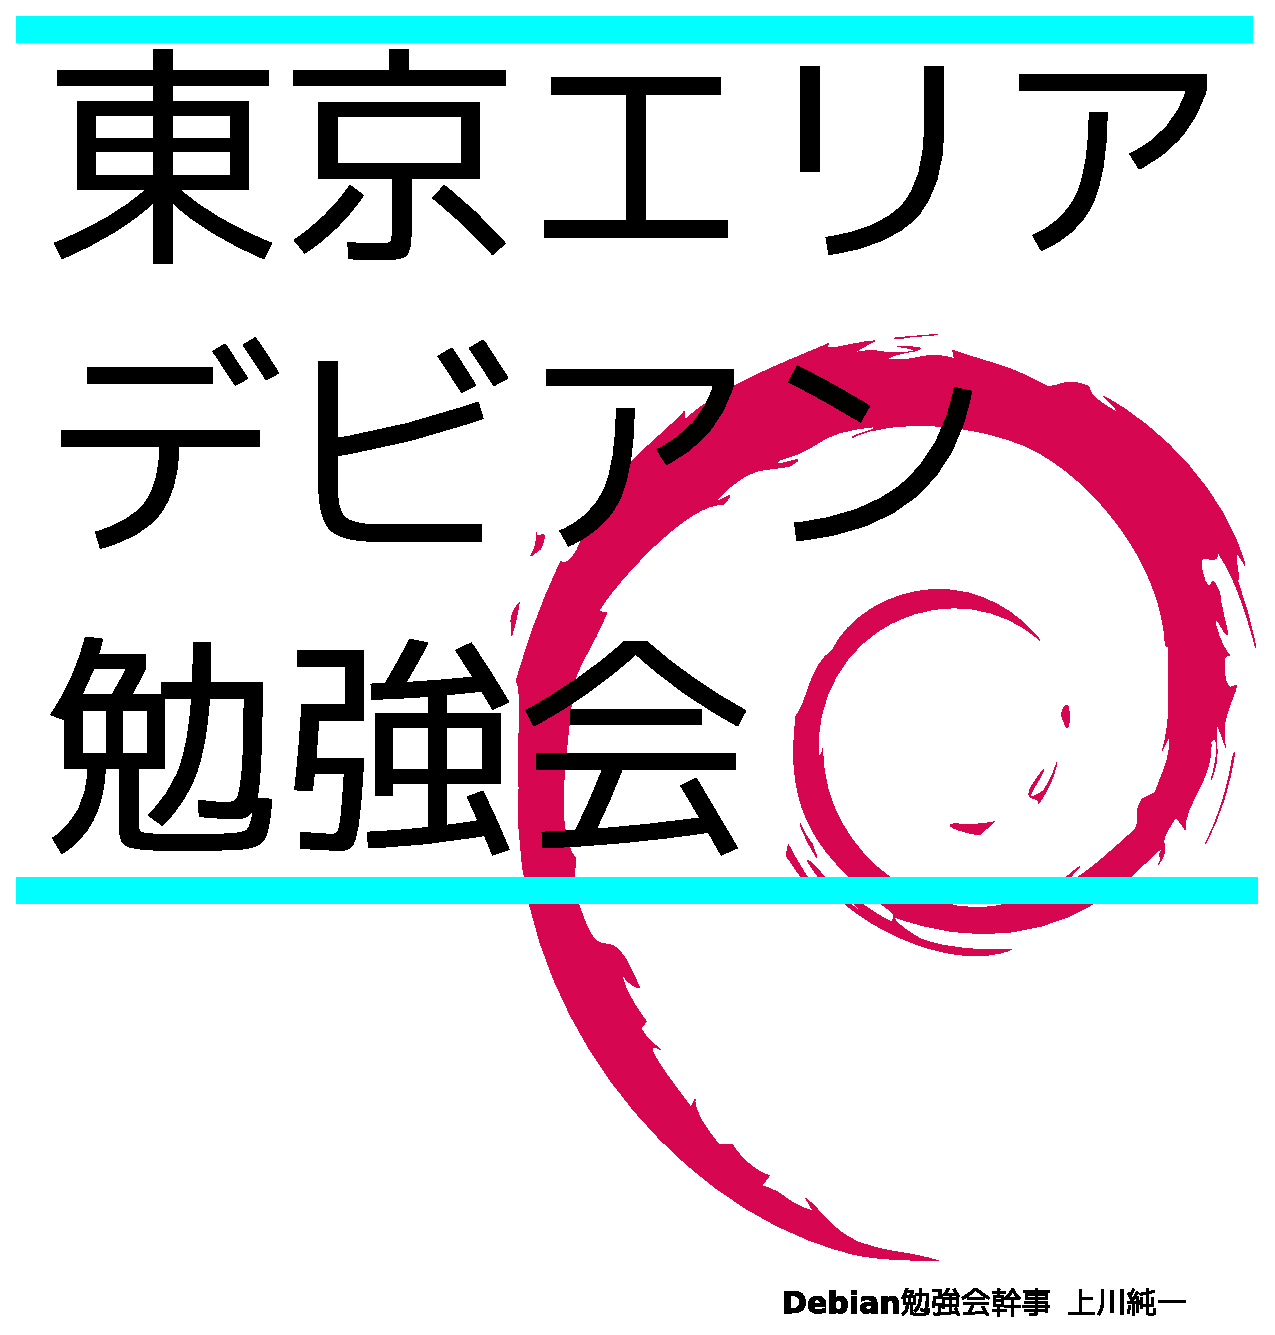
\includegraphics[width=210mm]{image200801/2008title.eps}\\
\hfill{}\debmtgyear{}$BG/(B\debmtgmonth{}$B7n(B\debmtgdate{}$BF|(B

\end{titlepage}


\dancersection{Introduction}{$B>e@n(B $B=c0l(B}

\begin{multicols}{2}
 
 
 $B:#7n$N(BDebian$BJY6/2q$X$h$&$3$=!#$3$l$+$i(BDebian$B$N@$3&$K$"$7$rF'$_F~$l$k$H(B
 $B$$$&J}$b!"$9$G$K$I$C$W$j$H$D$+$C$F$$$k$H$$$&J}$b!"7n$K0l2s(BDebian$B$K$D$$(B
 $B$F8l$j$^$;$s$+!)(B

 Debian$BJY6/2q$NL\E*$O2<5-$G$9!#(B

 \begin{itemize}
 \item \underline{Debian Developer} ($B3+H/<T(B)$B$N0i@.!#(B
 \item $BF|K\8l$G$N!V(B\underline{$B3+H/$K4X$9$k>pJs(B}$B!W$r@0M}$7$F$^$H$a!"%"%C%W%G!<%H$9$k!#(B
 \item \underline{$B>l(B}$B$NDs6!!#(B
 \begin{itemize}
  \item $BIaCJ$P$i$P$i$J>l=j$K$$$k?M!9$,(B face-to-face $B$G=P2q$($k>l$rDs6!(B
	$B$9$k!#(B
  \item Debian $B$N$?$a$K$J$k$3$H$r8l$k>l$rDs6!$9$k!#(B
  \item Debian$B$K$D$$$F8l$k>l$rDs6!$9$k!#(B
 \end{itemize}
 \end{itemize}		

 Debian$B$NJY6/2q$H$$$&$3$H$G5f6KE*$K$O;22C<TA40w$,(BDebian Package$B$r$,$j$,$j(B
 $B$H:n$k%9!<%Q!<%O%C%+!<$K$J$C$?;Q$rLQA[$7$F$$$^$9!#>pJs$N6&M-!&3hMQ$rDL$7(B
 $B$F(B Debian$B$N:#8e$NG=F0E*$JE83+$X$NEZBf$H$7$F!"!V>l!W$H$7$F$N6u4V$rDs6!$9(B
 $B$k$N$,L\E*$G$9!#(B

 2009$BG/$N7W2h$O2>$G$9!#(B

 \begin{enumerate}
  \item $B?7G/$N4k2h(B ($B%"%s%5%s%V%k2.7&3+:E(B)
  \item OSC Tokyo
  \item VAIO P $B%$%s%9%H!<%k5-O?!"(B
	$B%+!<%M%kFI=q2q!!%G%#%9%H%j%S%e!<%7%g%sBg=89g(B($B>.NS$5$s(B)($BEl5~Bg3X(B?)
  \item Git Handson ($B4d>>(B)($B$"$s$5$s$V$k2.7&(B?)
  \item $B2H(BDebian$B%5!<%P(B vs $B?&>l$N%M%C%H%o!<%/(B($B@iBeED6hETN)?^=q4[(B?\footnote{\url{http://www.library.chiyoda.tokyo.jp/}})
  \item Asterisk ($BEl5~Bg3X(B?)
  \item $B%9%Z%$%s$K$F3+:E(B
  \item Debconf$BJs9p2q(B
  \item OSC Fall?
  \item udev + HAL($B4d>>$5$s(B)
  \item 3D graphics $B3+H/!JF#Bt$5$s!K(B 
  \item Debian $B%5!<%P(B+VMware + $B3F<o(BOS$B!"(B
	$BB>$N2>A[2=%D!<%k(B(vserver etc.)$B!"(B
	$BK:G/2q(B
 \end{enumerate}

 $B2q>l8uJd$H$7$F$O2<5-$,$"$j$^$9(B:

 \begin{itemize}
  \item $BBg3X(B
  \item $B7CHf<w(BSGI$B%[!<%k(B
  \item Google$B%*%U%#%9(B
  \item $B8xL14[(B($B$"$s$5$s$V$k2.7&Ey(B)
  \item $BETN)2q5D<<(B($BL5@~(BLAN)
  \item $B7rJ]$N;\@_(B
 \end{itemize}

\end{multicols}

\newpage

\begin{minipage}[b]{0.2\hsize}
 \definecolor{titleback}{gray}{0.9}
 \colorbox{titleback}{\rotatebox{90}{\fontsize{80}{80} {\gt $B%G%S%"%sJY6/2q(B} }}
\end{minipage}
\begin{minipage}[b]{0.8\hsize}
\hrule
\vspace{2mm}
\hrule
\tableofcontents
\vspace{2mm}
\hrule
\end{minipage}

\dancersection{$B;vA02]Bj(B}{$B>e@n(B $B=c0l(B}

$B:#2s$N;vA02]Bj$O0J2<$G$9(B:

\begin{enumerate}
 \item 2009$BG/$r?6$jJV$C$F<+J,$O2?$r$7$?$+(B
 \item 2009$BG/$r?6$jJV$C$F(BDebian$B4XO"$G@$4V$G$O2?$,5/$3$C$?$+(B
\end{enumerate}

$B$3$N2]Bj$KBP$7$FDs=P$$$?$@$$$?FbMF$O0J2<$G$9!#(B

%; whizzy-master ../debianmeetingresume200912.tex
% $B0J>e$N@_Dj$r$7$F$$$k$?$a!"$3$N%U%!%$%k$G(B M-x whizzytex $B$9$k$H!"(Bwhizzytex$B$,MxMQ$G$-$^$9!#(B

\begin{prework}{$B>e@n=c0l(B}
\preworksection{2009$BG/$r?6$jJV$C$F<+J,$O2?$r$7$?$+(B}

2009$BG/!"H>J,$/$i$$$7$+(BDebian$BJY6/2q$K$O;22C$7$F$^$;$s!#(B

DDTSS $B$r$3$=$3$=$d$C$F$^$7$?$,!"5$$E$$$?$i:#G/$O(BDDTSS$B$N%5!<%P$,$H$^$C$?(B
 $B$j$H$$$m$$$m$H5/$-$?$h$&$G$9!#(B
%$BDI5-$9$k(B

\preworksection{2009$BG/$r?6$jJV$C$F(BDebian$B4XO"$G@$4V$G$O2?$,5/$3$C$?$+(B}

Netwalker $B$,%j%j!<%9$5$l$^$7$?$M!#(B
%$BDI5-$9$k(B

\end{prework}

\begin{prework}{$B5HED=SJe(B}
\preworksection{2009$BG/$r?6$jJV$C$F<+J,$O2?$r$7$?$+(B}
Debian$B4X78$@$H(BDDTSS$B$G%l%S%e!<$rCf?4$K(B180$B7oDxEY$d$C$F$$$?$h$&$G$9!#(B
DDTSS$B$O5Y$s$@$j$d$C$?$j!"$^$C$?$j$d$C$F$$$^$9!#(B
$B%$%Y%s%H4XO"$G$O(B2$B7n$K(BLinux conf.au$B$K9T$C$F!"=)$O(BJLS$B$K%\%i%s%F%#%";22C!"(B
KOF$B$K9T$C$F4X@>(BDebian$B$NJ}$H%-!<%5%$%s$r$7$?$j$7$F$$$^$7$?!#(B
$B$"$H$ONcG/DL$j!)$"$s$I$-$e$a$s$F$C$I$G$S$"$s$N%4!<%9%H%(%G%#%?!<7sGd$j;R$H$7$F!"(B
$BK?=j$GJY6/2q;qNA$r$^$H$a$FK\$K$7$FHRI[$7$F$$$^$9!#(B
\preworksection{2009$BG/$r?6$jJV$C$F(BDebian$B4XO"$G@$4V$G$O2?$,5/$3$C$?$+(B}
$B$d$O$j(BLenny$B%j%j!<%9$,0lHV$G$7$g$&!#(B
$B4pK\E*$K(Bstable$B$r;H$&%A%-%s$J$N$G!"%a%8%c!<%P!<%8%g%s%"%C%W$OBg$-$J(B
$B%K%e!<%9$G$9!#(B
$B:G6a$N(BDebian$B$ODj4|E*$K%j%j!<%9$5$l$k$N$G3F<o%=%U%H$b%P!<%8%g%s$,(B
$B3d$H?7$7$/!"JXMx$K46$8$F$$$^$9!#(B
$B$*$+$2$G;H$$$?$$%=%U%H$N$?$a$K!"(Bsid$BEy$+$i%P%C%/%]!<%H$7$?$j!"(B
$B$=$N$[$+(Btar$B%\!<%k$+$i%S%k%I$9$kI,MWEy$b>/$J$/$J$j!"$^$?$=$N>l9g$N<j4V$b(B
$B@N(B(woddy$B$N:"(B)$B$KHf$Y$F$+$J$j8:$C$F$*$j$"$j$,$?$$$G$9!#(B
\end{prework}



\dancersection{$B:G6a$N(BDebian$B4XO"$N%_!<%F%#%s%0Js9p(B}{$B$^$($@$3$&$X$$(B}
\subsection{$BEl5~%(%j%"(BDebian$BJY6/2q(B58$B2sL\Js9p(B}
% (query-replace-regexp "<.*?>" "")
% (query-replace-regexp "^[	 ]\+" "")

$BEl5~%*%j%s%T%C%/@D>/G/Am9g%;%s%?!<$G3+:E$7$^$7$?!#;22C<T$O!"$"$1$I$5$s!"(B
$B$J$+$*$5$s!"5HED$5$s!"$d$^$M$5$s!";3K\$5$s!"K\>1$5$s!"F|HfLn$5$s!"$"$i$-(B
$B$5$s!"9b66(B(emasaka)$B$5$s!"$D$8$?$5$s!"4d>>$5$s!"$^$($@$N(B12$BL>$G$7$?!#(B

Debian $B$G$N?t3X$3$H$O$8$a$H$7$F!"(Bgnuplot, Octave, R$B$NF~Lg$K$D$$$F$NOC$r(B
$B$^$($@$,9T$$$^$7$?!#(Bgnuplot $B$H(B R $B$G$N%W%m%C%H$N$d$jJ}$H!"(BR $B$H(B Octave $B$N(B
$B$=$l$>$l$N3HD%%Q%C%1!<%8$G$"$k(B CRAN, Octave-Forge $B$+$i$N(B Debian $B%Q%C%1!<(B
$B%82=$9$k$?$a$N%]%$%s%H%]%$%s%H$K$D$$$F5DO@$G$-$?$N$G!";22C$5$l$?J}$O(B
gnuplot $B$H(B R$B$r<+=,$7$F;H$($k$h$&$K$J$k$HF1;~$K!"(BOctave-Forge $B$H(B CRAN $B$N(B
$B3HD%%Q%C%1!<%8$r%,%s%,%s(B Debian $B%Q%C%1!<%8$K$9$k$Y$/(B ITP $B$7$F$$$k$3$H$G(B
$B$7$g$&!#(B

$B$b$&0l$D$N%M%?$H$7$F4d>>$5$s$,(B Debian auto-builder $B%M%C%H%o!<%/$K$D$$$F$N(B
$BOC$r$5$l$^$7$?!#(BDebian $B$r;Y$($k=EMW$J%7%9%F%`$G$"$k$K$b4X$o$i$:!"$3$N%7(B
$B%9%F%`$rM}2r$7$F$$$k(B DD $B$b>/$J$$$H$N$3$H$J$N$G!"$H$F$b0U5A$N$"$k%;%C%7%g(B
$B%s$G$7$?!#FC$K%I%-%e%a%s%H2=$5$l$F$$$J$$(B loop-depends $B$NBP1~$NOC$K$ON/0{(B
$B$r2<$m$7$??M$,B?$+$C$?$N$G$O$J$$$+$H;W$$$^$9!#:#2s$NOC$G!"(Bauto-builder
$B$K6=L#$r;}$C$?%R%H$O!"$<$R(B Debian/SH4$B$N%]!<%F%#%s%0$K;22C$7$^$7$g$&!#(B

$B1c2q$O!"@P11HT$-$?$F6>G~$H<r:h$NE9(B $B?4?h(B $B;25\66E9$K$F!#(BRolf $B$5$s$,1c2q$+(B
$B$i9gN.$5$l!"1c2q>l$G$N%-!<%5%$%s%Q!<%F%#$,9T$o$l$^$7$?!#(B

\subsection{Adam C Powell IV $B7^7b(B}
\begin{wrapfigure}{r}{18.5zw}
\includegraphics[width=1\hsize]{image200912/acp.jpg}
\end{wrapfigure}

11$B7n(B29$BF|$KMhF|$7$F$$$?(B Adam C Powell IV $B$r>e@n$,7^7b$7$^$7$?!#(B
Debian Beowulf Project $B$G@N$+$i$d$j$H$j$7$F$$$?Cg$G$9!#(B
$B=)MU86$K$$$C$FBg4n$S$7$F$$$^$7$?!#(B

$B$=$ND>A0$K(BDebian Developer$B$N9SLZ$5$s$H$b0l=o$K0{$_$K9T$C$F$$$?$h$&$G$9!#(B

\subsection{Dirk Eddelbuettel $B7^7b(B}

11$B7n(B26$BF|$KMhF|$7$F$$$?(B Dirk Eddelbuettel $B$r7^7b$7$^$7$?!#(Bgtach$B$5$s!"$@$$(B
$B$4$5$s!"4d>>$5$s!"A0ED$5$s!"(BDirk Eddelbuettel $BIW:J!">e@n(Bx2$B$K$F1c2q!#(B
Debian$B$H6bM;$K$D$$$FG.$/8l$k?7=I$NLk$G$7$?!#(B


% =======================================================================
\dancersection{$BEl5~%(%j%"(BDebian$BJY6/2q!!(B2009$BG/EY3F<o%$%Y%s%H3+:E<B@S$HAm3g(B}{$B>e@n(B $B=c0l(B}
\label{sec:debmtg2009results}
\index{debianjp@Debian JP} 
\index{$B$H$&$-$g$&$($j$"(B@$BEl5~%(%j%"(BDebian$BJY6/2q(B}
\index{2009$B$M$s(B@2009$BG/(B}

$B:#7n$G(B5$BG/L\$N(BDebian$BJY6/2q$,=*N;$7$^$7$?!#(B
Debian Developer$B$K$J$C$??M$,$$$?$jJQ2=$b$_$i$l!";d@83h$NLL$G$b(B
$B7k:'$7$?%a%s%P!<$,B??t$$$?$j!"(B
$BE>?&$7$?%a%s%P!<$,$$$?$j!"Ev;~$H=jB0$,JQ$o$C$F$$$J$$%a%s%P!<$N$[$&$,$a$:(B
$B$i$7$/$J$C$F$-$^$7$?!#(B

\subsection{Debian$BJY6/2q$NLnK>$N?JD=6q9g(B}

$B:#G/$O(BDebian$BJY6/2q$K$H$C$FBg$-$J$G$-$4$H$,$"$j$^$7$?!#(B
$BEv=i$NL\I8$G$"$C$?(BDebian Developer$B$N0i@.$H$$$&L\I8$,$9$3$7$E$D<B8=$7$F$-(B
$B$?$N$G$9!#El5~%(%j%"(BDebian$BJY6/2q>oO"$N4d>>$5$s!"4X@>(BDebian$BJY6/2qN)$A>e$2;~(B
$B4|$K?TNO$7$?Lp?a$5$s$,(BDebian Developer$B$K$J$j$^$7$?!#6l@a(B5$BG/!#$*$a$G$H$&(B
$B$4$6$$$^$9!#(B

2009$BG/$^$G$O4pK\E*$J(BDebian$B3+H/<T$K$J$k$^$G$N4pK\E*$J65M\$N6&M-$rL\E*$K$d$C(B
$B$F$-$^$7$?!#$3$l$+$i$O>/$7J}8~@-$rJQ$($F3+H/$KI,MW$J<BA)E*$JFbMF$K%7%U%H(B
$B$7$F$$$C$F$h$$$+$H9M$($F$$$^$9!#(B2010$BG/$O%9%]%s%5!<!"(BNMU$B!"(BBSP$B$N9T$$J}$r$h(B
$B$j<BA)E*$K9T$($kJ}8~$rLO:w$7$?$$$H;W$$$^$9!#(B

\subsection{$B1?1DJ}K!(B}

2009$BG/$NJY6/2q$K$O>e@nH>J,$/$i$$$7$+=P@J$7$F$*$i$:!"(B
$B4d>>!&A0ED$,Cf?4$H$7$F1?1D$K$"$?$j$^$7$?!#(B

$B;vA02]Bj$O(B latex $B$N%=!<%9%3!<%I$KBP$9$k(B git format-atch $B$N=PNO$r(BML$B$KEj9F(B
$B$9$k$H$$$&<j=g$G!"1c2q7/$H(B atnd $B$rJd=uE*$KMxMQ$7$^$7$?!#(B
$BJY6/2q2q>l$NM=Ls$O$H$j$"$($:(B30$B?M$/$i$$$,F~$l$k>l=j$r3NJ]$7$^$7$?$,!"(B
$B1c2q2q>l$NM=Ls$O?M?t$N3NDj$9$k3+:EFsF|A0!"$G$7$?!#(B

$BJY6/2q$N2qHq$O(B500$B1_$r0];}$7$F$$$^$9!#2a5n2.7&$N!V$"$s$5$s$V$k2.7&!W$H$$$&(B
$B8xL14[$rMxMQ$7$F$$$?$N$G!"HqMQ7W;;$b$=$3$r4p=`$K$*$3$J$C$F$-$F$$$^$7$?!#(B
2009$BG/$O$$$m$$$m$J2q>l$r;n$7$F$*$j!"8x1D$G$O$J$$;\@_$b;n$7$F$*$j!"2q>lHq(B
$BMQ$N9bF-$K$H$b$J$$@V;z7h;;$K$J$C$?2s$b$"$j$^$9!#8x1D$N;\@_$rMxMQ$7$F$$$k(B
$B$H2q>l$,Hs>o$K0B$+$C$?$N$G0u:~HqMQ$,$^$+$J$($F$$$^$7$?!#(B

$B44;v$O:rG/$^$G$O>e@n$,=8CfE*$K$7$F$$$?$N$G1?1D$K$D$$$F$N%N%&%O%&$,==J,EA(B
$B$o$C$F$$$J$+$C$?6lO+$b$"$C$?$_$?$$$G$9!#(B

\subsection{$B4pK\E*$J?tCM(B}

Debian $BJY6/2q$OKh2s;vA02]Bj;v8e2]Bj$r@_Dj$7$F$*$j!"M==,I|=,$rI,MW$@$H$&(B
$B$?$C$F$$$kJY6/2q$G$9!#(B
$B<B:]$K$I$l$/$i$$$N?M$,=P@J$7$F$$$k$N$+!"$^$?$=$N?M$?$A$,$I$l$/$i$$;vA02](B
$BBj!&;v8e2]Bj$rDs=P$7$F$$$k$N$+!"3NG'$7$F$_$^$7$g$&!#(B
\fgref{fig:attendandprepostwork}$B$G$9!#(B
$BCM$O0lG/$N0\F0J?6Q$G$9!#(B

\begin{figure}[ht]
 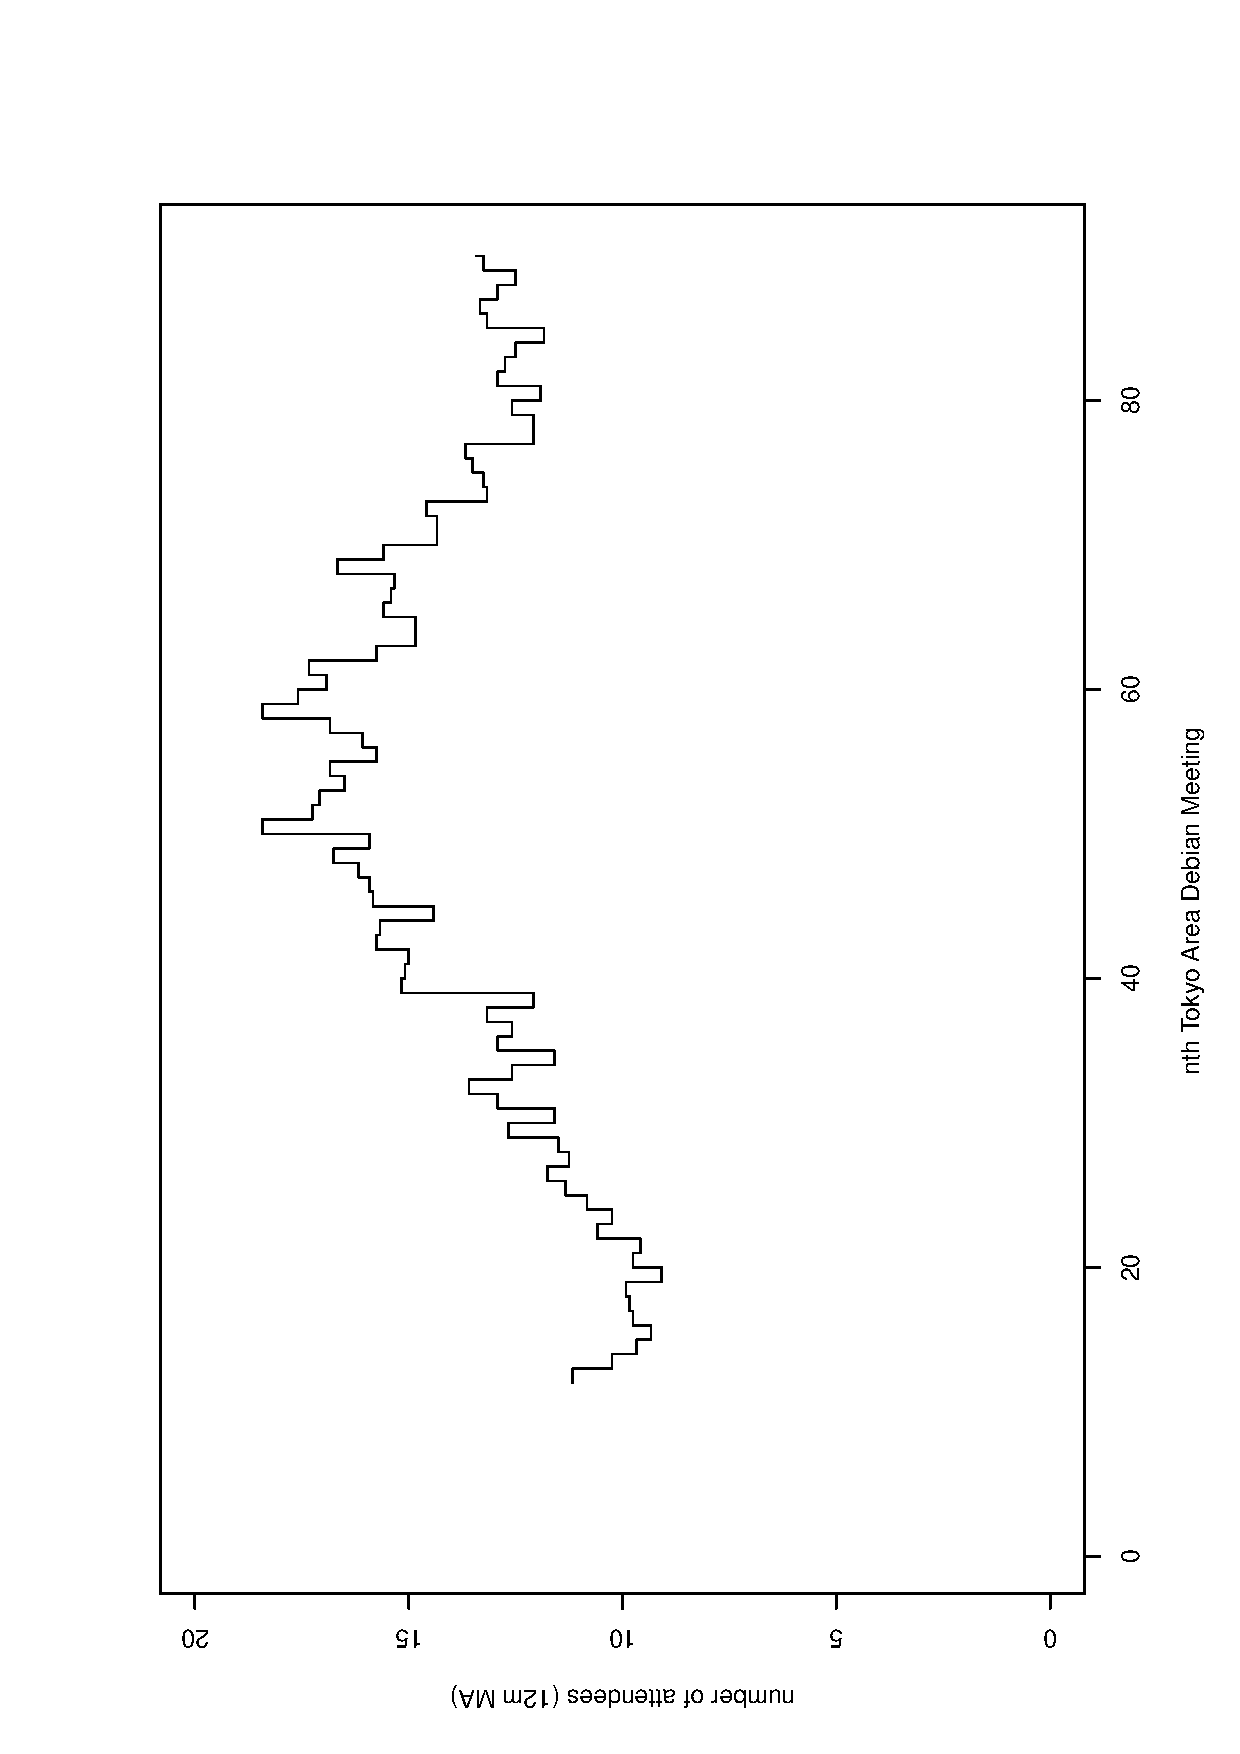
\includegraphics[width=1\hsize]{image200912/memberanalysis/attend.png}
\caption{$BEl5~%(%j%"(BDebian$BJY6/2q;vA02]Bj!&;v8e2]BjDs=P<B@S(B(12$B%v7n0\F0J?6Q(B)}\label{fig:attendandprepostwork}
\end{figure}

$BKh2s$N;22C<T$N?M?t$H!"$=$N:]$N%H%T%C%/$r8+$F$_$^$9!#:#G/$N>l9g$O!"J?F|$N(B
$BLk$K9T$C$?(BGPG$B%-!<%5%$%s%Q!<%F%#!<$N;22C<T$NB?$5$,L\N)$C$F$$$^$9!#(B
 
\begin{table}[ht]
\begin{minipage}{0.5\hsize}
 \caption{$BEl5~%(%j%"(BDebian$BJY6/2q;22C?M?t(B(2005-2006$BG/(B)}\label{tab:count}
 \begin{center}
  \begin{tabular}{|l|c|p{10em}|}
 \hline
   & $B;22C?M?t(B & $BFbMF(B \\
 \hline
   2005$BG/(B1$B7n(B & 21 & $BHkL)(B\\
   2005$BG/(B2$B7n(B & 10 & debhelper 1\\
   2005$BG/(B3$B7n(B & 8 &  ($BAaD+(B) debhelper 2$B!"(Bsocial contract\\
   2005$BG/(B4$B7n(B & 6 & debhelper 3\\
   2005$BG/(B5$B7n(B & 8 & DFSG$B!"(Bdpkg-cross$B!"(Blintian/linda\\
   2005$BG/(B6$B7n(B & 12 & alternatives$B!"(Bd-i\\
   2005$BG/(B7$B7n(B & 12 & toolchain$B!"(Bdpatch\\
   2005$BG/(B8$B7n(B & 7 & Debconf$B;22CJs9p!"(BITP$B$+$i%"%C%W%m!<%I$^$G(B\\
   2005$BG/(B9$B7n(B & 14 & debconf\\
   2005$BG/(B10$B7n(B & 9 & apt-listbugs$B!"%P%0%l%]!<%H!"(Bdebconf$BK]Lu!"(Bdebbugs\\
   2005$BG/(B11$B7n(B & 8 & DWN$BK]Lu%U%m!<!"(Bstatoverride\\
   2005$BG/(B12$B7n(B & 8 & $BK:G/2q(B\\
   2006$BG/(B1$B7n(B & 8 & policy$B!"(BDebian$BJY6/2q$G$d$j$?$$$3$H(B\\
   2006$BG/(B2$B7n(B & 7 & policy$B!"(Bmultimedia \\
   2006$BG/(B3$B7n(B & 30 & OSC: debian$BJY6/2q!"(Bsid \\
   2006$BG/(B4$B7n(B & 15 & policy$B!"(B\LaTeX{} \\
   2006$BG/(B5$B7n(B & 6 & mexico \\
   2006$BG/(B6$B7n(B & 16 & debconf$B!"(Bcowdancer\\
   2006$BG/(B7$B7n(B & 40 & OSC-Do: MacBook Debian \\
   2006$BG/(B8$B7n(B & 17 & 13$B<9G0(B \\
   2006$BG/(B9$B7n(B & 12 & $BK]Lu!"(BDebian-specific$B!"(Boprofile \\
   2006$BG/(B10$B7n(B & 23 & network$B!"(Bi18n$B2q5D!"(BFlash$B!"(Bapt \\
   2006$BG/(B11$B7n(B & 20 & $B4X@>3+:E!'(B bug$B!"(Bsid$B!"(Bpackaging \\
   2006$BG/(B12$B7n(B & 14 & $BK:G/2q(B \\
 \hline
  \end{tabular}
 \end{center}
\end{minipage}
\begin{minipage}{0.5\hsize}
 \caption{$BEl5~%(%j%"(BDebian$BJY6/2q;22C?M?t(B(2007-2008$BG/(B)}\label{tab:count2007}
 \begin{center}
  \begin{tabular}{|l|c|p{10em}|}
 \hline
 & $B;22C?M?t(B & $BFbMF(B\\
 \hline
   2007$BG/(B1$B7n(B & 15 & $B0lG/$r4k2h$9$k(B \\
   2007$BG/(B2$B7n(B & 13 & dbs, dpatch\\ 
   2007$BG/(B3$B7n(B & 80 & OSC$B2>A[2=(B \\
   2007$BG/(B4$B7n(B & 19 & quilt, darcs, git\\
   2007$BG/(B5$B7n(B & 23 & etch, pbuilder, superh \\   
   2007$BG/(B6$B7n(B & 4 & $B%(%8%s%P%i3+:E!'(BDebconf7 $B<B67Cf7Q(B \\
   2007$BG/(B7$B7n(B & 18 & Debconf7 $B;22CJs9p(B\\
   2007$BG/(B8$B7n(B & 25 & cdn.debian.or.jp \\   
   2007$BG/(B9$B7n(B & 14 & exim \\   
   2007$BG/(B10$B7n(B & 30 & OSC Tokyo/Fall(CUPS) \\   
   2007$BG/(B11$B7n(B & 19 & live-helper, tomoyo linux kernel patch, server\\
   2007$BG/(B12$B7n(B & 11 & $BK:G/2q(B\\
   2008$BG/(B1$B7n(B & 23 & $B0lG/$r4k2h$9$k(B \\
   2008$BG/(B2$B7n(B29+3$B7n(B1$BF|(B & 36 & OSC  \\
   2008$BG/(B3$B7n(B & 37 & $B%G!<%?$@$1$N%Q%C%1!<%8!"%i%$%;%s%9(B \\
   2008$BG/(B4$B7n(B & 17 & $B%P%$%J%j%Q%C%1!<%8(B \\
   2008$BG/(B5$B7n(B & 20 & $BJ#?t$N%P%$%J%j%Q%C%1!<%8(B \\
   2008$BG/(B6$B7n(B & 10 & debhelper \\
   2008$BG/(B7$B7n(B & 17 & Linux kernel patch / module $B%Q%C%1!<%8(B \\
   2008$BG/(B8$B7n(B & 10 & Debconf IRC$B2q5D$H(BDebian$B29@t(B \\
   2008$BG/(B9$B7n(B & 17 & po4a, $B!V(BDebian $B%a%s%F%J$N$*;E;v!W(B \\
   2008$BG/(B10$B7n(B & 11? & OSC Tokyo/Fall \\
   2008$BG/(B11$B7n(B & 17 & $B!V$=$N>l$GJY6/2q;qNA$r:n@.$7$A$c$(!W(B Debian $B$r;H$C$?(B \LaTeX{} $B869F:n@.9g=I(B \\
   2008$BG/(B12$B7n(B & 12 & $BK:G/2q(B \\
 \hline
  \end{tabular}
 \end{center}
\end{minipage}
\end{table}

\begin{table}[t]
\begin{minipage}{0.5\hsize}
 \caption{$BEl5~%(%j%"(BDebian$BJY6/2q;22C?M?t(B(2009$BG/(B)}\label{tab:count2009}
 \begin{center}
  \begin{tabular}{|l|c|p{10em}|}
 \hline
 & $B;22C?M?t(B & $BFbMF(B\\
 \hline
   2009$BG/(B1$B7n(B & 12 & $B0lG/$r4k2h$9$k(B \\
   2009$BG/(B2$B7n(B & 30 & OSC $B%Q%C%1!<%8%O%s%:%*%s(B\\ 
   2009$BG/(B3$B7n(B & 23 & Common Lisp, $B%Q%C%1!<%8:n@.(B \\
   2009$BG/(B4$B7n(B & 15 & Java Policy, ocaml, $B3+H/%o!<%/%U%m!<(B\\
   2009$BG/(B5$B7n(B & 13 & MC-MPI$B%Q%C%1!<%82=!"(BErlang$B!"(BAndroid$B%"%W%j!"(BDDTP \\   
   2009$BG/(B6$B7n(B & 14 & DDTP$B!&(BDDTSS$B!"(Bbsdstats$B%Q%C%1!<%8!"(BDebian kFreeBSD\\
   2009$BG/(B7$B7n(B & ? & $B%9%Z%$%s$K$F(BDebconf 9\\
   2009$BG/(B8$B7n(B & 14 & $B%9%Z%$%s(B Debconf 9 $B;22CJs9p(B \\   
   2009$BG/(B9$B7n(B & 26 & GPG$B%-!<%5%$%s%Q!<%F%#!<(B \\   
   2009$BG/(B10$B7n(B & ? & OSC Tokyo Fall\\
   2009$BG/(B11$B7n(B & 12 & Octave, R, gnuplot, auto-builder \\
   2009$BG/(B12$B7n(B & ? & $BK:G/2q(B\\
 \hline
  \end{tabular}
 \end{center}
\end{minipage}
\end{table}


%=================================================
\dancersection{$B4X@>(B Debian $BJY6/2q(B\newline2009$BG/EY3F<o%$%Y%s%H3+:E<B@S$HAm3g(B}{$BARI_!&:4!9LZ!&LnJ}(B}
\index{2009$B$M$s(B@2009$BG/(B}
\index{$B$+$s$5$$$G$S$"$s(B@$B4X@>(BDebian$BJY6/2q(B}

\subsection{$B1?1D>u67(B}

$B4X@>$O1?1D$K4X$o$C$F$$$k?M$K3X@8$,B?$$$N$G!"$$$m$$$mL5M}$r$*4j$$$9$k>l(B
$BLL$bB?$+$C$?$h$&$J5$$,$7$^$9!#(B

\subsubsection{$BJY6/2qA4BN(B}

$B:#G/EYESCf(B(7$B7n(B)$B$h$j!"1?1DC4Ev$,;32<B:Li$+$iARI_!&:4!9LZ!&LnJ}$N;0L>BN@)(B
$B$K8rBe$7$^$7$?!#$3$l$O;32<$N?HJU$,B?K;$K$J$j?HF0$-$,$H$l$J$$$H$$$&M}M3(B
$B$+$i$G$9!#9,$$!"0JA0$h$jJ,C4$K8~$11?1D$N8+D>$7$r?J$a$F$$$?$3$H$b$"$j!"(B
$BBg$-$J:.Mp$b$J$/7QB3$9$k$3$H$,$G$-$^$7$?!#(B

$BG/EYEv=i!"%i%$%VCf7Q$K<c43@9$j>e$,$j$r8+$;$^$7$?$,!"$=$N8e!"$&$^$/7QB3(B
$B$G$-$^$;$s$G$7$?!#LdBj$H$7$F$O(BIP$B%"%s%j!<%A%c%V%k$J2q>l$r%a%$%s$K$7$F$$(B
$B$k$3$H$H!"Cf7Q$N<B:n6H$rC4$C$F$$$??M$,1?1DB&$K%7%U%H$7!"M>NO$r2s$;$J$/(B
$B$J$C$F$$$k$3$H$,860x$H;W$o$l$^$9!#(B

5$B7n$K$O?@8M;T$rCf?4$H$7$?4X@>CO0h$N?77?%$%s%U%k%(%s%6N.9T$K$h$j!"JY6/(B
$B2q$rCf;_$9$k=PMh;v$,$"$j$^$7$?!#(B
$B<R2qE*$JMW0x$K$h$jJY6/2q3+:E$NH=CG$rGw$i$l$k>u67$O=i$a$F$G$7$?$,!"$3$&(B
$B$$$&;v$OFsEY$H$"$C$FM_$7$/$J$$$G$9$M!#(B

9$B7n$O5~ET%j%5!<%A%Q!<%/$K$*<YKb$7$FJY6/2q=i$N5~ET$G3+:E$7$^$7$?!#2q>l$r(B
$BJQ$($k$H!"$$$D$b$H$O0c$&;22C<T$bA}$($k$N$G!"$?$^$K>l=j$rJQ$($k$N$b$h$$(B
$B$N$G$O$H;W$$$^$7$?!#(B

$B9V;U$K$D$$$F$O8=>u!"8GDj2=$7$F$$$kCf!"7QB3$7$F>oO";22C<T$X$N9V;U0MMj$r(B
$B$9$k$[$+$K!"(BDMC$B$r<h$jF~$l$?$j!"(BLT$BH/I=$b2DG=$J;22C<T<+8J>R2p$N>o@_$J(B
$B$I$r$*$3$J$$$^$7$?!#(B

LT$BH/I=2DG=$J;22C<T<+8J>R2p$O!"OCBj$K%P%j%(!<%7%g%s$,2C$o$C$?$J$I6=L#?<(B
$B$$$3$H$b$"$C$?H?LL!"G/EY8eH>$O4X@>$NJY6/2q;22C<T$b;22C$7$F$$$k(B Open
Street Map$B$K%H%T%C%/$r;}$C$F$$$+$l$F$7$^$C$?46$b$"$j!"$&$^$/%P%i%s%9$r(B
$B<h$kI,MW$,$"$j$=$&$G$9!#(B

$B$^$?!":#G/EY$O:4!9LZ!";32<$N(B 2 $BL>$,(B Package Maintainer $B$H$7$F(B
Debian $B$N(B New queue $B$K?7$7$/%Q%C%1!<%8$rAw$j9~$_$^$7$?!#MhG/$b(B
$B$3$NN.$l$r0];}$G$-$l$P$H;W$$$^$9!#(B

\subsubsection{$B07$C$?%F!<%^(B}

$BJY6/2q$NFbMF$H$7$F$O!"%Q%C%1!<%83+H/<+BN$K2C$($F!"(BDebian $B$NBN@)$K$^$D$o(B
$B$kOC(B(gpg $B$d(B mentors $B$J$I(B)$B$d!"<~JU%D!<%k$NMxMQ(B(bash $B$d(B reportbug $B$d(B gdb
$B$J$I(B)$B$r$H$j$"$2$^$7$?!#(B
$BMhG/EY$N%F!<%^$K$D$$$F$O!"G/KvG/;O$KAjCL$r$9$kM=Dj$r$7$F$$$^$9!#(B

$BK]Lu4XO"$G$O!"El5~$G$NN.$l$K>h$j(BDDTSS$B$N%O%s%:%*%s<B=,$r$7$^$7$?$,!"M=A[(B
$B30$KH?1~$,$"$j$^$7$?!#$b$H$b$H<{MW$,$"$C$?$N$+!"<B=,$7$?$3$H$G?H6a$K$J$C(B
$B$?$N$+!"$O$h$/$o$+$j$^$;$s$,!D!#(B

\subsubsection{$B%$%Y%s%H4XO"(B}
$BNcG/DL$j!"2F$N%*!<%W%s%=!<%9%+%s%U%!%l%s%9(BKansai@Kyoto(OSC)$B$H!"=)$N4X(B
$B@>%*!<%W%s%U%)!<%i%`(B(KOF)$B$K=PE8$7$^$7$?!#(B

$B%;%C%7%g%s$G$O!"(BOSC$B$G$OBg1:$5$s$K$h$k(BDebian GNU/kFreeBSD$B$K$D$$$F!"(BKOF$B$G(B
$B$OLp?a$5$s$K(BDD$B$K$J$k$^$G$N50@W$r$*OC$7$F$b$i$$$^$7$?!#(B
$BLp?a$5$s$O!"4X@>(BDebian$BJY6/2qN)$A>e$2$NN)Lr<T$J$N$G!"$G$-$l$PJY6/2q$K$b(B
$BMh$FM_$7$$$H$3$m$G$9$,!":G6a$O!"$J$+$J$+$4B?K;$GFq$7$$$H$N$3$H$G$9!#(B

$B$^$?!";M9q$G$O$8$^$C$?%*!<%W%s%U%)!<%9JY6/2q(B \footnote{
\url{http://openforce.project2108.com/}}$B$H!"2,;3$G$N%*!<%W%s%;%_%J!<(B
$B!w2,;3(B \footnote{\url{http://openseminar.okaya.ma/}} $B$K!"LnJ}$,;22C$7$F(B
Debian Live$B$d%N%&%O%&$N>R2p$J$I$r9T$$$^$7$?!#(B

\subsection{$B3+:E<B@S(B}

$B4X@>(BDebian$BJY6/2q$N=P@J>u67$r3NG'$7$F$_$^$7$g$&!#(B
$B%0%i%U$G8+$k$H(B\fgref{fig:kansaipeoplechart}$B$K$J$j$^$9!#(B
$BI=$G8+$k$H(B\tbref{tab:count2009kansai} $B$G$9!#(B

\begin{figure}[h]
 \begin{center}
  \includegraphics[width=1\hsize]{image200912/kansai.png}
 \end{center}
\caption{$B4X@>$N;22C?M?t?d0\(B}
\label{fig:kansaipeoplechart}
\end{figure}

\begin{table}
\begin{minipage}{0.5\hsize}
 \caption{$B4X@>(BDebian$BJY6/2q;22C?M?t(B(2007$BG/(B)}\label{tab:count2007kansai}
 \begin{center}
  \begin{tabular}{|l|c|p{10em}|}
 \hline
 & $B;22C?M?t(B & $BFbMF(B \\
 \hline
2007$BG/(B3$B7n(B & 19 & $B3+:E$K$"$?$j(B \\
2007$BG/(B4$B7n(B & 25 & goodbye$B!"(Byoutube$B!"%W%m%8%'%/%H%H%i%C%+!<(B\\
2007$BG/(B6$B7n(B & 23 & $B<R2q7@Ls!"%F!<%^!"(Bdebian/rules$B!"(Bbugreport\\
2007$BG/(B7$B7n(B & 20$BA08e(B & OSC-Kansai \\
2007$BG/(B8$B7n(B & 20 & Inkscape$B!"(Bpatch$B!"(Bdpatch\\
2007$BG/(B9$B7n(B & 16 & $B%i%$%V%i%j!"K]Lu!"(Bdebtorrent\\
2007$BG/(B10$B7n(B & 22& $BF|K\8lF~NO!"(BSPAM$B%U%#%k%?(B\\
2007$BG/(B11$B7n(B & 20$BA08e(B & KOF \\   
2007$BG/(B12$B7n(B & 15& $BK:G/2q!"(BiPod touch\\   
 \hline
  \end{tabular}
 \end{center}
\end{minipage}
\begin{minipage}{0.5\hsize}
 \caption{$B4X@>(BDebian$BJY6/2q;22C?M?t(B(2008$BG/(B)}\label{tab:count2008kansai}
 \begin{center}
  \begin{tabular}{|l|c|p{10em}|}
 \hline
 & $B;22C?M?t(B & $BFbMF(B \\
 \hline
2008$BG/(B2$B7n(B & 20 & PC Cluster, GIS, \TeX \\
2008$BG/(B3$B7n(B & 23 & bug report, developer corner, GPG \\
2008$BG/(B4$B7n(B & 24 & coLinux, Debian GNU/kFreeBSD, sid \\
2008$BG/(B5$B7n(B & 25  & ipv6, emacs, ustream.tv\\
2008$BG/(B6$B7n(B & 20  & pbuilder, hotplug, ssl\\
2008$BG/(B8$B7n(B & 13  & coLinux \\
2008$BG/(B9$B7n(B & 17  & debian mentors, ubiquity, DFSG\\
2008$BG/(B10$B7n(B & 11  & cdbs,cdn.debian.or.jp \\
2008$BG/(B11$B7n(B & 35  & KOF \\
2008$BG/(B12$B7n(B & ?  & TeX$B;qNA:n@.%O%s%:%*%s(B\\
 \hline
  \end{tabular}
 \end{center}
\end{minipage}
\begin{minipage}{0.5\hsize}
 \caption{$B4X@>(BDebian$BJY6/2q;22C?M?t(B(2009$BG/(B)}\label{tab:count2009kansai}
 \begin{center}
  \begin{tabular}{|l|c|p{10em}|}
 \hline
 & $B;22C?M?t(B & $BFbMF(B \\
 \hline
2009$BG/(B1$B7n(B & 18 & DMCK, LT \\
2009$BG/(B3$B7n(B & 12 & Git \\
2009$BG/(B4$B7n(B & 13 & Installing sid, Mancoosi, keysign \\
2009$BG/(B6$B7n(B & 18 & Debian Live, bash\\
2009$BG/(B7$B7n(B & 30? & OSC2009Kansai \\
2009$BG/(B8$B7n(B & 14 & DDTSS, lintian \\
2009$BG/(B9$B7n(B & 14 & reportbug, debian mentors\\
2009$BG/(B10$B7n(B & 16 & gdb, packaging \\
2009$BG/(B11$B7n(B & 35 & KOF2009 \\
2009$BG/(B12$B7n(B & ?? & GPS program, OpenStreetMap \\
 \hline
  \end{tabular}
 \end{center}
\end{minipage}
\end{table}

%=================================================
\dancersection{2009$BG/$r?6$jJV$C$F$_$k(B}{$B>e@n(B $B=c0l(B}
%=================================================
\index{2009$B$M$s(B@2009$BG/(B}

\subsection{$B:G6a$N%H%l%s%I$H:#8e$N?d0\(B}

$B:G6a$I$s$J$3$H$,(B
$B$"$C$F!"$3$l$+$i$I$&$$$&$3$H$,$"$k$G$7$g$&$+!#(B
$B$_$s$J$GM=A[$7$F$_$^$7$g$&!#(B

{\footnotesize
\begin{tabular}[t]{|p{8em}|p{8em}|p{12em}|p{8em}|p{8em}|}
\hline
2007 &2008 &2009 & 2010 & 2011 \\
\hline
%2007
VT$B!&(BAMD-V($B2>A[2=5;=Q(B)$B$,Ia5Z(B(ML115!)$B!"(B

$B8<H"(B(ARM)$B!"(B
OpenBlocks(PPC?)$B!"(B
iPhone$BEP>l!"(B 
HSDPA $B7n3[(B5000$B1_$/$i$$$K!"(B
google mobile$B!"(B

VISTA$B%j%j!<%9!"(B 
Leopard$B%j%j!<%9!"(B 

GPL3.0$B!"(B
$B%a%b%j(B2G$B$,%3%b%G%#%F%#!<$K!"(B
SparcT2$B$,%*!<%W%s!"(B 
$B%K%3%K%3F02h!"(B
& 
%2008
python 3.0
ruby 1.9

wine 1.0, wine64 $BEP>l(B

RoR 2.0 $BEP>l$GIa5Z$K(B

4$B%3%"!&(B64bit $B$N(BCPU$B$,%G%9%/%H%C%W$KIa5Z!"(B
Core2Quad $BCM2<$2!#(B

$B%K%3%K%3F02h(B1000$BK|%f!<%6FMGK!"(B
$B=i2;%_%/%V!<%`$K(B

$BCO%G%84XO"$N(BPC$B@=IJ$NIa5Z(B

$BJY6/2q$NIa5Z(B($B3ZE7$H$+(B)

$B8x=0L5@~(BLAN (wireless gate)

$B7HBSEEOC$NGd>e$,Mn$A$k!"(B
iPhone, Android $BEP>l!"(B
emobile 100$B1_(BPC$BJz$-$"$o$;(B
(eeePC, Dell mini9)
Zaurus$BHNGd=*N;!#(B

Chumby $BH/Gd!#(B

$B%5!<%P$N2>A[2=(B ESXi$B!&%7%s%/%i%$%"%s%H(B

MacBook Air $BH/Gd!"(B
$BL5@~(B 802.11n $B$,<B5!$K(B

SystemZ10 $BH/I=(B

$B@$3&7P:Q$NJx2u(B(IT$BEj;q6[=L:b@/!"?&$r<:$&?M$,A}2C(B)

FreeBSD 7 (malloc, ZFS ?)

Debian$B<!@$Be0i@.7W2h;OF0(B

Debian Maintainer $B@)EY;OF0(B

$B%;%-%e%j%F%#!<4XO"(B(OpenSSL $B;v7o!"(BDNS$B;v7o(B)

$B%/%i%&%I4XO"$,N.9T(B?

Nintendo DSi

&
%2009
$B@/8"8rBe(B,$B%9%Q%3%s;v6H;EJ,$1(B,$B1_9b(B

Windows7,Snow Leopard$BH/Gd(B

Netwalker$BH/Gd(B

MacBook$B$+$i(BIEEE1394$B$,>C$($?!#(B

$B%a%b%j$,(BDDR3$B$K0\9TCf(B,$B%a%b%j9bF-(B

$B%^%8%3%sHNGd<h$jDy$^$j(B

$B%i%V%W%i%9(B,OSS$B$r;H$C$?%(%m%2!<EP>l(B(OpenCV),AR,$B%;%+%$%+%a%i(B

JLS$B$G(BLinus$BMh$FBgA{$.(B

DD,2$B@$CB@8(B

$B%G%8%?%k%5%$%M!<%8(B

Google Voice,Wave,Chrome,Chrome OS,Go,$BF|K\8lF~NO(B,$BELJb%J%S(B

CouchDB

Twitter,*$B$J$&%V!<%`(B

Eye-Fi,Kindle2,DS LL,PSP-GO,POKEN

Cell$B=*N;$N$*CN$i$;(B

tile window manager boom ?

Lenny $B%j%j!<%9(B

Debian $B7k:'%V!<%`(B

$B%G%9%/%H%C%W!"(B4$B%3%"!"(B8GB

$B%N!<%H%Q%=%3%s!"(B2$B%3%"!"(B4GB

Linux $B$,I8=`%$%s%9%H!<%k$N(BPC$B!#(B(Dell)

SSD $B$NCMCJ$HMFNL$,$3$J$l$k(B($B$^$"$^$"(B)
HDD$B$,$J$/$J$k(B?$B9b$/$J$k(B?($B$J$i$:(B)

SSD$BFC2=$7$?(BFS$B$,=P$F$-$?(B

ipv6 $B;H$($k$h$&$K$J$C$F$k(B($BMhG/(B)

DL$B6X;_K!(B? torrent $B$K5UIw(B?

&
%2010
Debian OAuth$B%5!<%S%93+;O$N$*CN$i$;(B

SolidICE$B;H$C$?(BDebian VDI$B%5!<%S%93+;O$N$*CN$i$;(B

Chrome OS,Android$BE}9g$N$*CN$i$;(B

Willcom$B=*N;$N$*CN$i$;(B

Netbook,$B%/%i%&%I(B,Ameba$B$J$&=*N;$N$*CN$i$;(B

Debian Cloud$B%j%j!<%9$N$*CN$i$;(B

10GbE,SSD$BIa5Z(B

$B?7(BiPhone$B%j%j!<%9(B

$B<+L1I|3h(B

SIM$B%m%C%/%U%j!<1d4|$N$*CN$i$;(B

$B?7(BAndroid$BC<Kv(B($BF|K\0J30(B)

$B<!@$BeMQ(BFS:btrfs,NILFS

Lenny and Half$B%j%j!<%9(B

Squeeze$B%j%j!<%9CY1d(B,kFreeBSD,SH4 $B%*%U%#%7%c%k%"!<%-%F%/%A%c$K(B

ToyStory3$B%j%j!<%9(B

$B>CHq@G>e>:$KH<$&HKK;4|(B

$B%/%i%&%I$K$h$j!"C1=c$J%[%9%F%#%s%06H<T$,$D$E$+$J$$(B?
$B0lIt$O<+<R$G$b$D$h$&$K$J$k(B?

USB 3.0 $BEk:\!"(Bwireless USB vs Bluetooth ?

$BAH$_9~$_(BCPU$B$O(BAtom$B$KE}0l(B?Arm$B$O;D$C$F$k(B?

ruby 2.0 $B%j%j!<%9(B?Perl6$B%j%j!<%9(B?

&
%2011
Windows$B%I%i%$%P%7%0%K%A%c%A%'%C%/$,$J$/$J$k(B

IEEE1394$B=*N;$N$*CN$i$;(B

LTE$B$,=y!9$KIa5Z(B

$BCO%G%81d4|$N$*CN$i$;(B

Debian 11 $BF|K\3+:E(B

Google$B$KE}9g(B($B%*%U%#%9%=%U%H!"%0%k!<%W%&%'%"!"%a!<%k!"%U%!%$%k%5!<(B
		 $B%P;_$a$h$&$<1?F0(B)

Scala$B$N%(%s%?!<%W%i%$%:MxMQ(B

Windows11$B%j%j!<%9(B

C/S$B$r0U<1$;$:$K%"%W%j3+H/$G$-$k4D6-(B($B%3%s%Q%$%i$,<+F0H=CG(B)

\\

\hline
\end{tabular}

}

\clearpage

%=================================================
\dancersection{qemubuilder 2009$BG/%"%C%W%G!<%H(B}{$B>e@n=c0l(B}
%=================================================
\label{sec:qemubuilder-update2009}
\index{$B2>A[2=(B} 
\index{ARM} 
\index{qemu}
\index{qemubuilder}

\subsection{qemubuilder$B$N4pK\%3%s%;%W%H(B}

qemubuilder $B$O(BDebian$B%Q%C%1!<%8$r%S%k%I$9$k$?$a$N%D!<%k$G$9!#(Bdebootstrap$B$N(B
$B%/%m%9%V!<%H%9%H%i%C%W5!G=$rMxMQ$7$F%Y!<%9%$%a!<%8$r:n@.$7$?8e!"(Bqemu $B$rMx(B
$BMQ$7$F3F%"!<%-%F%/%A%cMQ$N2>A[%^%7%s$r<B9T$7!"$=$NCf$G%Q%C%1!<%8$r%S%k%I(B
$B$7$^$9!#%M%$%F%#%V%S%k%I$HJQ$o$i$J$$;HMQ46$G%Q%C%1!<%8$N%S%k%I$,$G$-$k$N(B
$B$GLLE]$J%/%m%9%S%k%I$N@_Dj$,I,MW$"$j$^$;$s!#FC$K(BDebian$B%Q%C%1!<%8$O(Bbuildd
$B$G%M%$%F%#%V%S%k%I$5$l!"%/%m%9%S%k%I$5$l$J$$A0Ds$J$N$G!"(Bbuildd$B$G%S%k%I$G(B
$B$-$k$h$&$J%Q%C%1!<%8$N:n@.!&%G%P%C%0$KJXMx$G$9!#(B

\subsection{qemubuilder$B$N;H$$J}(B}

$BMxMQ$7$?$$%"!<%-%F%/%A%c8~$1$N%+!<%M%k$H@_Dj%U%!%$%k$rMQ0U$7$^$9!#(B
$B<j85$N@_Dj$G$O<!$N$h$&$J@_Dj$K$J$C$F$$$^$9!#(B
\begin{commandline}
KERNEL_IMAGE=vmlinuz-2.6.24-1-versatile-armel
ARCH=armel
BASEPATH=/home/dancer/tmp/base-armel.qemu
INITRD=
\end{commandline}

$B%$%a!<%8$r$^$::n@.$7$^$9!#$3$l$G!"(BBASEPATH$B$K;XDj$7$?%U%!%$%kL>$K(Bqemu$B$N(B
RAW$B%G%#%9%/%$%a!<%8$,:n@.$5$l$^$9!#(B

\begin{commandline}
# qemubuilder --configfile arm.config --create 
\end{commandline}

$B%G%#%9%/%$%a!<%8$r%"%C%W%G!<%H$7$^$9!#(B

\begin{commandline}
# qemubuilder --configfile arm.config --update
\end{commandline}

$B%Q%C%1!<%8$r%S%k%I$9$k$N$K$O(B dsc $B%U%!%$%k$r;XDj$7$^$9!#(B

\begin{commandline}
# qemubuilder --configfile arm.config --build xxx.dsc
\end{commandline}

\subsection{qemubuilder$B$N2]Bj(B}

$B%+!<%M%k$H@_Dj%U%!%$%k$N<hF@$,:#0lHVLLE]$J$H$3$m$G$9!#(BDebian$B$NI8=`$N%+!<(B
$B%M%k$H(B initrd $B$G$G$-$?;~4|$b$"$C$?$N$G$9$,!"8=:_$=$&$$$&$h$&$K$O$J$C$F$$(B
$B$^$;$s!#(B

$B%"!<%-%F%/%A%c$NAH$_9g$o$;$,$"$^$j$K$bB?$$$?$a!"F0$/AH$_9g$o$;$rF1Dj$9$k(B
$B$3$H$d!"%G%P%C%0$,:$Fq$G$9!#%9%/%j%W%H$G<+F02=$9$k$3$H!"$^$?%F%9%H$N<+F0(B
$B2=$,I,MW$G$O$J$$$+$H9M$($F$$$^$9!#(B

$B$^$?!"(Bqemu $B$N(B-append$B%3%^%s%I$G%+!<%M%k$K%V!<%H%Q%i%a!<%?$r;XDj$G$-$k$3$H(B
$B$rAuCz$7$F$$$^$9$,!"<B:]$K$O$=$l$,$G$-$J$$%"!<%-%F%/%A%c(B(ppc$B$J$I(B)$B$,$"$j!"(B
$B$=$N$^$^$G$OF0$-$^$;$s!#(B\footnote{$B$$$^$G$b$=$&$+$O$o$+$j$^$;$s(B}

$B:G6a$O(BkFreeBSD$B%"!<%-%F%/%A%c$J$I$bEP>l$7$F$-$F$$$^$9$,!"$3$N$^$^$N@_7W$G(B
$B$O$=$3$^$G<j$,2s$i$J$5$=$&$G$9!#(B

\subsection{qemubuilder$B$N:#8e$N?J$aJ}(B}

$B$I$&$7$^$7$g$&$M!#(B

%=================================================
\dancersection{lxc $B%3%s%F%J$r;H$C$F$_$k(B }{$B$^$($@$3$&$X$$(B}
\label{sec:lxc}
\index{$B$+$=$&$+(B@$B2>A[2=(B} 
\index{Linux Kernel Container}
\index{Containers}
\index{lxc}

Debian $BJY6/2q$K;22C$5$l$F$$$kLL!9$O!"$=$m$=$m(B Xen $B$d(B KVM $B0J30$K2?$+$J$$(B
$B$N$+!"?7$?$J%M%?$r5a$a$F$$$k8~$-$,B?$$$+$H;W$$$^$9!#$=$3$G!":G6a!"(BLinux
Kernel $B$K?7$?$K%^!<%8$5$l$?5!G=$r;H$C$F<B8=$7$F$$$k!"(Blxc $B$H$$$&2>A[2=5;(B
$B=Q$K$D$$$F>R2p$7$^$9!#(B

\subsection{$B$O$8$a$K(B}
\subsubsection{lxc $B$N35MW(B}
lxc\footnote{\url{http://lxc.sourceforge.net/}} $B$O!"@5<0L>>N$r(B Linux
Containers $B$H8@$$!"%3%s%F%J<+BN$,2TF/$9$k$?$a$N%+!<%M%k$N5!G=$H!"%3%s%F(B
$B%J$r4IM}$9$k$?$a$N$H%f!<%6%D!<%k$+$i9=@.$5$l$^$9!#(Blxc $B$G;HMQ$7$F$$$k(B
Kernel $B$N5!G=(B(Control Group, $B0J2<(B Cgroup$B!!$H>JN,(B)$B$O!"(B
kernel 2.6.29 $B$G40A4$K%^!<%8$5$l!"%+!<%M%k$K%Q%C%A$rEv(B
$B$F$F%S%k%I$9$kI,MW$,$J$/$J$C$F$J$C$F$$$^$9!#(Bkernel 2.6.29 $B$h$jA0$N%+!<%M(B
$B%k$G$O!"(Bkernel 2.6.27 $B0J9_$G$"$l$P%Q%C%A$rEv$F$l$P;H$&$3$H$,(B
$B$G$-$^$9!#(B

lxc $B$O(B GPL2 $B%i%$%;%s%9$G8x3+$5$l$F$$$F!"3+H/$*$h$S%a%s%F%J%s%9$O!"(BDaniel
Lezcano $B;a$,<B<A0l?M$G9T$C$F$$$^$9!#(B

Debian $B$G$O!"(BSqueeze/Sid $B$+$i%Q%C%1!<%82=$5$l$F$*$j!"0l$DA0$N:G?7HG(B
\footnote{2009$BG/(B11$B7n(B27$BF|8=:_!"(B0.6.3$B!#(B}$B$,%Q%C%1!<%8$H$J$C$F$$$^$9!#(B

\subsubsection{$BB>$N%3%s%F%J7?2>A[2=5;=Q$H$NHf3S(B}

$B%3%s%F%J7?$N2>A[2=5;=Q$H$$$&$HM-L>$J$N$O!"(BSolaris Containers $B$d(B FreeBSD
jail$B$,$"$j$^$9$,!"(BLinux $B$G$O(B Linux-VServer, OpenVZ\footnote{Parallels
Virtuozzo Containers$B$N(BOSS$BHG!#(B}$B$J$I$,$"$j$^$9!#$$$:$l$b4{$K;H$C$?$3$H$,$"(B
$B$kJ}$,B?$$$N$G$O$J$$$N$G$7$g$&$+!#(B

lxc $B$GDs6!$5$l$k%5!<%S%9$O!"Bg$-$/J,N`$7$F%7%9%F%`%3%s%F%J$H!"%"%W%j%1!<%7%g%s%3%s%F%J$N(B2
$B$D$,$"$j$^$9!#A0<T$O!"$$$o$f$k(BOS$B$^$k$4$H$N2>A[2=$G$9!#(Binit $B$+$i5/F0$7$F!"2>A[(BOS
$B$N6u4V$rDs6!$7$^$9!#8e<T$O!"(Bchroot $B$K$h$k%"%W%j%1!<%7%g%s$NJ,N%$K6a$$$G(B
$B$9!#C10l%"%W%j%1!<%7%g%s$rJ,N%$9$k$@$1$J$N$G!"$H$F$b7Z$/%7%s%W%k(B
$B$J$N$,FCD'$G$9!#(B

lxc $B$O8=>u!"0l?M$G3+H/!&%a%s%F%J%s%9$5$l$F$*$j!":#8e%W%m%8%'%/%H(B
$B$,$I$&$J$k$N$+@h9T$-8+$($J$$$H$3$m$G$O$"$j$^$9!#8=:_!"%a!<%j%s%0%j%9%H$r8+(B
$B$F$$$k8B$j$G$O3+H/$OB3$$$F$$$k$h$&$G$9!#(B

\subsection{$BF3F~$7$F$_$k(B}
\subsubsection{$B%=!<%9%3!<%I$r<hF@$9$k(B}
$B%f!<%6%9%Z!<%9$N%D!<%k$N%=!<%9%3!<%I$O!"(BSourceForge $B$K$"$j$^$9!#(B
$B%=!<%9%3!<%I$O(B git $B$G4IM}$5$l$F$*$j!":G?7HG$O(B git $B%j%]%8%H%j$+$i<hF@$G$-$^$9!#(B

\begin{commandline}
$ git clone git://lxc.git.sourceforge.net/gitroot/lxc/lxc
\end{commandline}

Debian $B$G$OA0=R$N$H$*$j!"(BSqueeze/Sid $B$G%Q%C%1!<%8$K$J$C$F$$$k(B
\footnote{\url{http://packages.debian.org/search?keywords=lxc&searchon=names&exact=1&suite=all&section=all}}
$B$?$a!":G?7HG$G$"$kI,MW$,$J$1$l$P!"%=!<%9%3!<%I$OFC$KI,MW$"$j$^$;$s!#(B

\subsubsection{$B%+!<%M%k%*%W%7%g%s$rM-8z$K$9$k(B}
lxc $B$N5!G=$r%U%k$K3hMQ$9$k$K$O0J2<$N%+!<%M%k%*%W%7%g%s$,M-8z$K$J$C$F$$$k(B
$BI,MW$,$"$j$^$9!#(B

\begin{commandline}
* General
  * Control Group support
    -> namespace cgroup subsystem
    -> cpuset support
    -> Group CPU scheduler
    -> control group freeze subsystem
    -> Basis for grouping tasks (Control Groups)
    -> Simple CPU accounting
    -> Resource counters
    -> Memory resource controllers for Control Groups
    -> Namespace support
    -> UTS namespace
    -> IPC namespace
    -> User namespace
    -> Pid namespace
  * Network support
    -> Networking options
      -> Network namespace support
\end{commandline}

$B$3$l$i$,M-8z$K$J$C$F$$$k$+$r3NG'$9$k$K$O!"(Blxc$B$N%=!<%9%D%j!<$K4^$^$l$F$$$k!"(B
src/lxc/lxc-checkconfig.in $B$H$$$&%7%'%k%9%/%j%W%H$r<B9T$9$l$P!"8=:_5/F0(B
$BCf$N%+!<%M%k$G$I$N%+!<%M%k%*%W%7%g%s$,L58z$K$J$C$F$$$k$+$r%A%'%C%/$G$-$^(B
$B$9!#(B

$B$^$?!"(BDebian $B%Q%C%1!<%8$G$O!"(B/usr/bin/lxc-checkconfig $B$H$7$F%$%s%9%H!<%k(B
$B$5$l$F$$$^$9!#(BSqueeze/Sid $B$G(B Debian $B$N%+!<%M%k%Q%C%1!<%8(B\footnote{2009$BG/(B
11$B7n(B27$BF|8=:_!"(Blinux-image-2.6.30-2-amd64}$B$r;H$C$F$$$k4D6-$G3NG'$9$k$H0J(B
$B2<$N7k2L$K$J$j$^$9!#(BCgroup memory controller $B$N$_$,L58z$K$J$C$F$$$k$h$&(B
$B$G$9!#(B

\begin{commandline}
$ lxc-checkconfig 
Kernel config /proc/config.gz not found, looking in other places...
Found kernel config file /boot/config-2.6.30-2-amd64
--- Namespaces ---
Namespaces: enabled
Utsname namespace: enabled
Ipc namespace: enabled
Pid namespace: enabled
User namespace: enabled
Network namespace: enabled
Multiple /dev/pts instances: enabled

--- Control groups ---
Cgroup: enabled
Cgroup namespace: enabled
Cgroup device: enabled
Cgroup sched: enabled
Cgroup cpu account: enabled
Cgroup memory controller: disabled
Cgroup cpuset: enabled

--- Misc ---
Veth pair device: enabled
Macvlan: enabled
File capabilities: enabled
\end{commandline}

\subsubsection{Debian $B$G$N%$%s%9%H!<%k(B}

$B$3$3$+$i@h$O!"(BSqueeze/Sid $B$G%Q%C%1!<%8$r;H$&$3$H$rA0Ds$H$7$FOC$r?J$a$^$9(B
$B$,!"$3$N$^$^$G$O!"(Bcgroup $B$G$N%a%b%j4IM}$OL58z$K$J$C$F$$$^$9$N$G!"%+!<%M(B
$B%k%*%W%7%g%s(B \verb!CONFIG_CGROUP_MEM_RES_CTLR! $B$rM-8z$K$7$F%j%S%k%I$7$F$/$@$5$$!#(B
$B$=$l0J30$G<B:]$K(B Debian $B$G(B lxc $B$r;H$&$?$a$KI,MW$J%Q%C%1!<%8$O2?$+$H$$$&$H(B
lxc $B$@$1$G$9!#(B

\begin{commandline}
$ sudo apt-get install lxc
\end{commandline}

$B$3$l$G%"%W%j%1!<%7%g%s%3%s%F%J$r;n$9$3$H$O$G$-$^$9!#(BREADME $B$K$b:\$C$F$$(B
$B$k<j=g$G$9$,!"<!$N%3%^%s%I$r<B9T$9$k$H!"B(@J$N%3%s%F%J$r5/F0$G$-$^$9!#(B

\begin{commandline}
$ uname -a
Linux silicon 2.6.32 #1 SMP Sun Dec 6 02:30:30 JST 2009 x86_64 GNU/Linu
$ sudo lxc-execute -n hoge -f ./lxc-macvlan.conf /bin/bash
# uname -a
Linux alpha 2.6.32 #1 SMP Sun Dec 6 02:30:30 JST 2009 x86_64 GNU/Linux
\end{commandline}

$BB>$N%3%s%=!<%k$+$i%3%s%F%J$,5/F0$7$F$$$k$+3NG'$7$F$_$^$9!#(B

\begin{commandline}
$ sudo lxc-info -n hoge
'hoge' is RUNNING
$ lxc-ps -n hoge 
CONTAINER    PID TTY          TIME CMD
            4747 pts/3    00:00:00 bash
            5692 pts/3    00:00:00 lxc-ps
            5693 pts/3    00:00:00 ps
\end{commandline}

$B$A$c$s$H3NG'$G$-$^$7$?$M!#:#2s$O!"$3$l$G0J>e$G$9!"$H8@$$$?$$$H$3$m$G$9$,!"(B
$B$3$N4D6-$O%3%s%F%J$r5/F0$5$;$?$@$1$G$7$+$J$/!"$O$C$-$j8@$C$FLr$KN)$A$^$;(B
$B$s!#(Bbash $B$r(B sudo $B$G5/F0$7$F$$$k$@$1$G!"%[%9%H(B OS $B$N%U%!%$%k%7%9%F%`$K$b(B
$B%"%/%;%9$G$-$F$7$^$$$^$9!#(B

$B%3%s%F%J$@$1$r5/F0$5$;$FK~B-!"$O$$!"=*N;$H$9$k$N$G$"$l$PNI$$$+$b$7$l$^$;(B
$B$s$,!"<B:]$K(B lxc $B$r3hMQ$7$h$&$H9M$($F$$$k$J$i<!$K5s$2$kB>$N%Q%C%1!<%8$r(B
$B%$%s%9%H!<%k$7!"$5$i$K%3%s%F%JMQ$N%/%m!<%:4D6-$r:n$kI,MW$,$"$j$^$9!#(B

\begin{itemize}
 \item iproute : $B%3%s%F%J$N%M%C%H%o!<%/@_Dj$r9T$&$?$a!#(B
 \item debootstrap : $B%3%s%F%J$N%$%a!<%8$r:n@.$9$k$?$a!#(B
\end{itemize}

$B:#2s$O!"%/%m!<%:$J(B Debian $B4D6-$r4JC1$K:n$k$?$a$NJ}K!$r>R2p$7$^$9!#(B
\footnote{$B87L)$K8@$&$H!"%3%s%F%J$+$i%[%9%H(B OS $B$G2TF/$7$F$$$k%W%m%;%9$d!"(B
$B%+!<%M%k%a%C%;!<%8$,8+$($F$7$^$&$N$G%/%m!<%:$K$O$^$@$J$C$F$$$k$H$O8@$($^(B
$B$;$s$,!"$^$@3+H/Cf$G$b$"$k$N$G$=$N$&$A2~A1$5$l$k$G$7$g$&!#(B}

\subsubsection{$B%M%C%H%o!<%/$N@_Dj(B}
\subsubsubsection{\textbf{$B%V%j%C%8$N@_Dj(B}}

$BI,MW$J%Q%C%1!<%8$r%$%s%9%H!<%k$7$?$i!"$^$:$O%V%j%C%8$N@_Dj$r9T$&I,MW$,$"$j$^$9!#(B
/etc/network/interfaces $B$GD>@\%V%j%C%8$N@_Dj$r$9$l$PNI$$$H;W$$$^$9$,!#%7%'(B
$B%k%9%/%j%W%H$rMQ0U$7$F!"$=$l$r(Bpost-up $B$G<B9T$5$;$l$PNI$$$G$7$g$&!#(B

\begin{commandline}
#!/bin/sh

brctl addbr br0                             <- $B%V%j%C%8%G%P%$%9$NDI2C(B
brctl setfd br0 0                           <- $B%V%j%C%8%G%P%$%9(B br0 $B$N@_Dj(B
ifconfig br0 192.168.0.1 promisc up
brctl addif br0 eth0
ifconfig eth0 0.0.0.0 up
route add -net default gw 192.168.0.254 br0 <- $B%[%9%H(B OS $B$N%2!<%H%&%'%$(B
\end{commandline}

interfaces $B$O0J2<$N$h$&$K@_Dj$7$^$9!#(B
\begin{commandline}
$ cat /etc/network/interfaces 
# This file describes the network interfaces available on your system
# and how to activate them. For more information, see interfaces(5).

# The loopback network interface
auto lo
iface lo inet loopback

# The primary network interface
auto eth0
allow-hotplug eth0
iface eth0 inet static
	address 192.168.0.101
	netmask 255.255.255.0
	broadcast 192.168.0.255
	pre-up  /etc/init.d/iptables start
	post-up /etc/network/if-up.d/brctl.sh
\end{commandline}

$B0J>e$N$"$H!"%V%j%C%8$N@_Dj$,$-$A$s$H$5$l$F$$$k$+3NG'$7$F$_$k$H!"0J2<$N$h(B
$B$&$K$J$j$^$9!#(B
\begin{commandline}
$ /usr/sbin/brctl show
bridge name	bridge id		STP enabled	interfaces
br0		8000.00wwwwyyyyxxno		eth0
							veth0_14820
							veth0_15932
							veth0_17164
\end{commandline}
$B$A$J$_$K(B``veth0\_''$B$N8e$m$N?t;z$O!"%3%s%F%J$G5/F0$7$?(B init $B%W%m%;%9$N%W%m%;%9(BID
$B$G$9!#(B


\subsubsubsection{\textbf{IP $B%U%)%o!<%I$H(B NAT $B$N@_Dj(B}}

$B%[%9%H(B OS $B$H%3%s%F%J!"%3%s%F%J$H%[%9%H(B OS $B$N30It$N%M%C%H%o!<%/!"%3%s%F%J(B
$B4V$G$NDL?.$O!">e5-$N@_Dj$@$1$G$J$/!"(BIP $B%U%)%o!<%I$d(B NAT $B$N@_Dj$r$9$kI,MW(B
$B$,$"$j$^$9!#Nc$($P!"%3%s%F%J5/F08e!"%[%9%H(B OS $B$+$i(B ssh $B$G%m%0%$%s$9$k$N(B
$B$K$b!"(BIP $B%U%)%o!<%I$,I,MW$H$J$j$^$9!#(B

\begin{commandline}
$ sudo bash -c ``echo 1 > /proc/sys/net/ipv4/ip_forward''
\end{commandline}

IP $B%U%)%o!<%I$r@_Dj$9$k$H$H$G!"%[%9%H(B OS $B$N30It$N%M%C%H%o!<%/$X$NDL?.$d!"(B
$B%3%s%F%JF1;N$NDL?.$b9T$($k$h$&$K$O$J$j$^$9!#(B\footnote{$BF1$8%V%m!<%I%-%c%9(B
$B%H%I%a%$%s$N>l9g!#(B}

$B0lJ}!"%[%9%H(B OS $B$N30It%M%C%H%o!<%/$+$i$O$3$N$^$^$G$O%"%/%;%9$G$-$^$;$s!#(B
$B%"%/%;%9$r5v2D$9$k$K$O!"%[%9%H(B OS $B$G%]!<%H%U%)%o!<%G%#%s%0$d!"08@h(B NAT$B$J(B
$B$I$r9T$&I,MW$,$"$j$^$9!#%]!<%H%U%)%o!<%G%#%s%0$r9T$&$N$G$"$l$P!"0J2<$N$h(B
$B$&$J%k!<%k$r@_Dj$7$^$9!#(B

\begin{commandline}
iptables -t nat -A PREROUTING -d 192.168.0.1 -p tcp --dport 80 -i br0 -j DNAT --to 192.168.0.101
iptables -t nat -A PREROUTING -d 192.168.0.1 -p tcp --dport 5984 -i br0 -j DNAT --to 192.168.0.102
\end{commandline}

$B$3$3$G$N@_Dj$O!"%G%U%)%k%H%]%j%7!<$,A4$F(B ACCEPT$B$G$"$k$3$H$rA0Ds$K$7$F$$(B
$B$^$9$,!"<B:]$K$OEvA3(B DROP $B$K$9$k$H;W$$$^$9$N$G!"(BFORWARD $B$N%k!<%k$J$I$bDj(B
$B5A$9$kI,MW$,$"$j$^$9!#(BNetfilter $B$N%k!<%k$H(BIP$B%U%)%o!<%G%#%s%0$N5v2D$O%9%/(B
$B%j%W%H$K$7$F!"(B/etc/network/interface $B$G(B pre-up $B$H$7$F@_Dj$7$F$*$/$HNI$$(B
$B$G$7$g$&!#(B

$B$J$*!"(BFORWARD $B%A%'%$%s$N%G%U%)%k%H%]%j%7!<$,(B ACCEPT $B$G$"$k>l9g$OLdBj$"$j(B
$B$^$;$s$,!"(BDROP $B$d(B REJECT $B$K@_Dj$7$F$"$k>l9g$O!"%3%s%F%JF1;N$G$NDL?.$O$G(B
$B$-$^$;$s!#(BFORWARD $B%A%'%$%s$G$N(B ACCEPT $B%k!<%k$,I,MW$K$J$j$^$9!#(B

\subsubsection{$B%7%9%F%`%3%s%F%J$N:n@.(B}
\label{sec:make_container}

$B$G$O!"%7%9%F%`%3%s%F%J$N%$%a!<%8$r:n@.$7$F$_$^$9!#(Blxc $B$N%Q%C%1!<%8$K4^$^$l$k!"(B
/usr/share/doc/lxc/examples/lxc-debian.gz $B$r;H$C$F!"(BDebian $B$N%7%9%F%`%3(B
$B%s%F%J$r:n@.$7$^$9!#(B

$B$^$:!"$3$N%U%!%$%k$r%[!<%`%G%#%l%/%H%j$J$I$G?-D%$7$^$9!#(B
\begin{commandline}
$ zcat /usr/share/doc/lxc/examples/lxc-debian.gz > ~/lxc-debian
\end{commandline}

$B<!$K!"(Bcgroup $B%U%!%$%k%7%9%F%`$r%^%&%s%H$7$^$9!#(B/etc/fstab $B$K2<5-0l9T$rDI(B
$B5-$7$^$9!#%^%&%s%H%]%$%s%H$OG$0U$N>l=j$G9=$$$^$;$s!#(B

\begin{commandline}
cgroup  /var/local/cgroup  cgroup  defaults  0  0
\end{commandline}

$BDI5-$7$?$i!"%^%&%s%H%]%$%s%H$N%G%#%l%/%H%j$r:n@.$7!"%^%&%s%H$7$^$9!#(B

\begin{commandline}
$ sudo mkdir /var/local/cgroup
$ sudo mount cgroup
\end{commandline}

$B$=$l$G$O!"@h$[$I$N(B lxc-debian $B%9%/%j%W%H$r;H$C$F%3%s%F%J%$%a!<%8$r:n@.$7(B
$B$^$9!#$3$N%9%/%j%W%H$G$O(B debootstrap $B$r;H$C$F%$%a!<%8$,:n@.$5$l$^$9$,!"(B
$B%G%#%9%H%j%S%e!<%7%g%s$O(B lenny $B$K$J$C$F$$$^$9!#A0=R$7$?DL$jK\4D6-$O(B
Squeeze/Sid $B$G$9$N$G!"%3%s%F%J$b(B Squeeze/Sid $B$NJ}$,NI$1$l$P!"%3%s%F%J%$(B
$B%a!<%8$r:n@.$9$kA0$KM=$a%9%/%j%W%H$r=q$-49$($F$*$/I,MW$,$"$j$^$9!#(B
$B$^$?!"%Q%C%1!<%8$b!"%G%U%)%k%H$G(B apache2 $B$,%$%s%9%H!<%k$5$l$?$j!"0lJ}!"(B
sudo $B$d(B vi, dig $B%3%^%s%I$,L5$+$C$?$j$9$k$N$G!"$=$N$^$^%$%s%9%H!<%k$9$k$H(B
$BITJX$G$"$C$?$j$9$k$N$G!"M=$a%$%s%9%H!<%k$9$k%Q%C%1!<%8$N;XDj$rJQ99$7$F$*(B
$B$/I,MW$,$"$j$^$9!#(Blxc-debian $B%9%/%j%W%HFb$N(B debootstrap $B%3%^%s%I$N(B
\verb/--include/$B%*%W%7%g%s$G%Q%C%1!<%8$N;XDj$OJQ99$G$-$^$9!#(B
$B$^$?!"(Bsshd $B$N@_Dj$d!"%M%C%H%o!<%/$N@_Dj$bM=$a@_Dj$7$F$*$/$HJXMx$G$9!#0J(B
$B2<!"JQ99:Q$_%U%!%$%k$H$N(B diff $B$N7k2L$r7G:\$7$F$*$-$^$9!#(B

\begin{commandline}
$ diff -u  a/lxc-debian b/lxc-debian 
--- a/lxc-debian	2009-11-30 21:22:59.000000000 +0900
+++ b/lxc-debian	2009-10-30 17:58:20.000000000 +0900
@@ -8,8 +8,8 @@
 MNTFILE=
 TMPMNTFILE=
 UTSNAME=
-IPV4="172.20.0.21"
-GATEWAY="172.20.0.1"
+IPV4="192.168.0.101"
+GATEWAY="192.168.0.1"
 MTU="1500"
 
 # These paths are within the container so do not need to obey configure prefixes
@@ -99,14 +99,14 @@
 SyslogFacility AUTH
 LogLevel INFO
 LoginGraceTime 120
-PermitRootLogin yes
+PermitRootLogin no
 StrictModes yes
 RSAAuthentication yes
 PubkeyAuthentication yes
 IgnoreRhosts yes
 RhostsRSAAuthentication no
 HostbasedAuthentication no
-PermitEmptyPasswords yes
+PermitEmptyPasswords no
 ChallengeResponseAuthentication no
 EOF
 }
@@ -259,8 +259,8 @@
 	        # download a mini debian into a cache
 		echo "Downloading debian minimal ..."
 		debootstrap --verbose --variant=minbase --arch=$ARCH \
-		    --include ifupdown,locales,libui-dialog-perl,dialog,apache2,netbase,net-tools,iproute,openssh-server \
-		    lenny $CACHE/partial-$ARCH http://ftp.debian.org/debian
+		    --include ifupdown,locales,libui-dialog-perl,dialog,sudo,vim-tiny,dnsutils,netbase,net-tools,iproute,openssh-server \
+		    sid $CACHE/partial-$ARCH http://cdn.debian.or.jp/debian
 		
 		RESULT=$?
 		if [ "$RESULT" != "0" ]; then
\end{commandline}

$B$=$l$G$O!"%3%s%F%J$r:n@.$7$^$9!#%3%s%F%J$r:n@.$9$k>l=j$OG$0U$N>l=j$K$G$-(B
$B$^$9!#DL>o!"(Blxc-debian $B%9%/%j%W%H$r<B9T$r<B9T$7$?%G%#%l%/%H%j$N2<$K(B
debian$B%G%#%l%/%H%j$r<+F0E*$K:n@.$7!"$=$N2<$K%3%s%F%J%$%a!<%8$G$"$k(B
rootfs $B$,:n@.$5$l$^$9!#G[CV$7$?$$%G%#%l%/%H%j$,L5$1$l$P:n@.$7!"$=$N%G%#(B
$B%l%/%H%j$X0\F0$7!"(B\texttt{sudo lxc-debian create}$B$r<B9T$7$^$9!#(B

\begin{commandline}
$ sudo mkdir /var/cache/lxc
$ cd /var/cache/lxc
$ sudo bash /home/kohei/lxc-debian create
What is the name for the container ? [debian] hoge                 <- $B%3%s%F%J$NL>A0(B
What hostname do you wish for this container ? [hoge]              <- $B%3%s%F%J$N%[%9%HL>(B
What IP address do you wish for this container ? [192.168.0.101]   <- $B%3%s%F%J$N(B IP$B%"%I%l%9(B
What is the gateway IP address ? [192.168.0.1]                     <- $B%3%s%F%J$+$i8+$?%G%U%)%k%H%2!<%H%&%'%$$N%"%I%l%9(B
What is the MTU size ? [1500]
Specify the location of the rootfs [./rootfs.hoge]
Specify the location for an extra fstab file [(none)]
(snip)
Choose your architecture
1) amd64
2) i386
#? 1                                                               <- Core 2 Duo $B$N%^%7%s$J$N$G%"!<%-%F%/%A%c$O(B amd64 $B$rA*Br!#(B
Architecture amd64 selected
Checking cache download ...Found.
Copying rootfs ...Done.
(snip)
update-rc.d: using dependency based boot sequencing
Done.

You can run your container with the 'lxc-start -n hoge'
\end{commandline}

$B$3$l$G!"(B/var/cache/lxc/debian/rootfs.hoge $B$H$$$&L>A0$G%3%s%F%J%$%a!<%8$N(B
$B%G%#%l%/%H%j$,:n@.$5$l!"$3$3$K!"(Bdebootstrap $B$K$h$k(B Debian $B%$%a!<%8$N%3%T!<(B
$B$,:n@.$5$l$^$9!#=i$a$F(B \texttt{lxc-debian create} $B$r<B9T$9$k$H!"(B
debootstrap $B$G%@%&%s%m!<%I$5$l$k%-%c%C%7%e%$%a!<%8$,!"(B
/var/cache/lxc/debian/rootfs-architecture $B$H$7$F:n@.$5$l$^$9!#(B\footnote{$B:#2s$O(B
amd64 $B$rA*Br$7$F$$$k$N$G!"(B/var/cache/lxc/debian/rootfs-amd64 $B$H$J$j$^$9!#(B}

$B%3%s%F%J<+BN$N%a%?>pJs$O!"(B/var/lib/lxc $B%G%#%l%/%H%j$N%3%s%F%JL>$N%G%#%l(B
$B%/%H%j0J2<$K$"$j$^$9!#%D%j!<I=<($9$k$H0J2<$N$h$&$K$J$C$F$$$^$9!#(B

\begin{commandline}
$ tree hoge/
couchdb/
|-- cgroup
|-- config
|-- fstab
|-- init
|-- network
|   `-- veth0
|       |-- ifindex
|       |-- link
|       |-- mtu
|       |-- name
|       `-- up
|-- nsgroup -> /var/local/cgroup/hoge
|-- pts
|-- rootfs
|   `-- rootfs -> /var/cache/lxc/debian/rootfs.hoge
|-- state
|-- tty
`-- utsname

5 directories, 13 files
\end{commandline}

\subsubsection{$B%7%9%F%`%3%s%F%J$N5/F0(B}

$B%7%9%F%`%3%s%F%J$N5/F0$NA0$K!"$d$k$3$H$,$"$j$^$9!#%3%s%F%J%$%a!<%8$K!"%m(B
$B%0%$%s2DG=$J%f!<%6%"%+%&%s%H$r:n@.$9$k$3$H$H!"(B/etc/hosts $B$r=q$-49$($k$3(B
$B$H$G$9!#A0<T$O!"%3%s%F%J:n@.8e$K$=$N$^$^5/F0$5$;$?$N$G$O!"%m%0%$%s$9$k$3(B
$B$H$,$G$-$^$;$s!#%[%9%H(BOS $BB&$HF1$8%f!<%6%"%+%&%s%H$GLdBj$J$1$l$P!"(B
/var/cache/lxc/debian/rootfs.hoge/etc/$B%G%#%l%/%H%j$N2<$N!"(Bpasswd,
shadow, group $B$r%[%9%H$N$=$l$G>e=q$-$7$F$*$/$HNI$$$G$7$g$&(B\footnote{$B:#8e(B
$B:n@.$9$k%3%s%F%JA4$F$K6&DL$7$F8@$($k$3$H$J$N$G!"%-%c%C%7%e%$%a!<%8$G$"$k!"(B
/var/cache/lxc/debian/rootfs-amd64/etc/$B%G%#%l%/%H%j0J2<$r>e=q$-$7$F$*$$(B
$B$?J}$,NI$$$+$b$7$l$^$;$s!#(B}$B!#8e<T$O%3%s%F%J<+?H$NL>A02r7h$N@_Dj$,L\E*$G(B
$B$9!#8=>u$G$O!"%3%s%F%J$N(B/etc/hosts $B$O!"0lN'!"(B

\begin{commandline}
127.0.0.1	localhost
127.0.1.1	$B%[%9%H(BOS$B$N%[%9%HL>(B
\end{commandline}

$B$H$J$C$F$*$j!">e5-$N(B2$B9TL\$,!"(B/etc/hostname $B$H0[$J$k$?$a!"%f!<%6%"%+%&%s(B
$B%H$r:n$C$F$b!"%m%0%$%s;~$KL>A02r7h$G;~4V$,3]$+$C$F$7$^$$$^$9!#(B
$B$G$9$N$G!"M=$a!"%[%9%H(BOS$B$N%[%9%HL>$K$J$C$F$$$kItJ,$r%3%s%F%J$N%[%9%HL>$K=q$-49$($F$*$/I,MW(B
$B$,$"$k$o$1$G$9!#(B\footnote{$B$3$l$O!"(Blxc-debian $B%9%/%j%W%H<+BN$G%3%s%F%J$N(B
$B%[%9%HL>$r=q$-49$($k$h$&$K$7$F$*$1$P:Q$`OC$@$H;W$&$s$G$9$1$I$M!#(B}

$B>e5-$N@_Dj$r=*$($?$i!"%7%9%F%`%3%s%F%J$r5/F0$7$^$9!#(B
$B%7%9%F%`%3%s%F%J$N5/F0$O!"(B\texttt{lxc-start} $B%3%^%s%I$r;H$$$^$9!#0l$D$N(B
$B4D6-$GJ#?t$N%3%s%F%J$r5/F0$G$-$k$N$G!"%3%s%F%JL>$N;XDj$,I,$:I,MW$G$9!#%3(B
$B%s%F%JL>$N;XDj$K$O!"%*%W%7%g%s(B\texttt{-n} $B$r;H$$$^$9!#(B

\begin{commandline}
$ sudo lxc-start -n hoge
\end{commandline}

$B$3$N$^$^5/F0$5$;$k$H!"8=:_$N%7%'%k$G$=$N$^$^%3%s%F%J$N%3%s%=!<%k$,I=<($5(B
$B$l$^$9!#%m%0%$%s$9$k$K$O$=$N$^$^%3%s%=!<%k%m%0%$%s$9$l$PNI$$$G$7$g$&!#(B
$B%P%C%/%0%i%&%s%I$G5/F0$5$;$k$K$O!"(B\texttt{-d} $B%*%W%7%g%s$r$D$1$^$9!#(B

\begin{commandline}
$ sudo lxc-start -n hoge -d
\end{commandline}

KVM $B$d(B Xen $B$J$I$N$h$&$K%+!<%M%k$+$i5/F0$5$;$kLu$G$O$J$/!"(Binit $B%W%m%;%9$+(B
$B$i5/F0$5$;$k$N$G!"5/F040N;$^$G$KMW$9$k;~4V$O$o$:$+$G$9!#(B

\subsection{lxc $B$N;EAH$_$r8+$F$_$k(B}
\subsubsection{$B%3%s%F%J$N%i%$%U%5%$%/%k(B}

Linux $B%3%s%F%J$N%i%$%U%5%$%/%k$OB>$N2>A[2=5;=Q$HBg$-$/0[$J$k$H$3$m$O$J$/!"(B
$B<!$N?^$NMM$K$J$j$^$9!#(B

\includegraphics[width=0.8\hsize]{image200912/lxc/lxc-lifecycle.eps}

$B$3$N?^$G$N>uBV$rA+0\$5$;$k$?$a$N%3%^%s%I!"$D$^$j%3%s%F%J$r4IM}$9$k$?$a$N(B
$B%3%^%s%I$O0J2<$NDL$j$G$9!#(B

{\footnotesize
\begin{tabular}[t]{|p{8em}|p{6em}|p{16em}|p{18em}|}
\hline
status &$B%3%^%s%I(B &$B<B9T8e$N>uBV(B &$BHw9M(B \\
\hline
\hline
$B%3%s%F%J$N5/F0(B &lxc-start &STARTING, RUNNING &$B%7%9%F%`%3%s%F%J(B \\
&lxc-execute & &$B%"%W%j%1!<%7%g%s%3%s%F%J(B\\
\hline
$B%3%s%F%J$N0l;~Dd;_(B &lxc-freeze &FROZEN & \\
\hline
$B%3%s%F%J$N:F3+(B &lxc-unfreeze &RUNNING & \\
\hline
$B%3%s%F%J$NDd;_(B &lxc-stop &STOPPING, STOPPED & \\
\hline
$B%3%s%F%J$N:F5/F0(B &lxc-restart &STOPPING, STOPPED & \\
& &STARTING, RUNNING & \\
\hline
$B%3%s%F%J$N:n@.(B &lxc-create &STOPPED &lxc-debian $B$OFbIt$G(Blxc-create $B$r<B(B
	     $B9T!#(B \\
& & &lxc-fedora, lxc-sshd$B$J$I$bF1MM!#(B \\
\hline
$B%3%s%F%J$NGK4~(B &lxc-destroy & & \\
\hline
\end{tabular}}

\subsubsection{$B%j%=!<%9$r@)8f$9$k(B}

lxc $B$G$O!"%3%s%F%J$N%j%=!<%9$r@)8f$9$k$?$a$K!"(Bcgroup $B$H$$$&%+!<%M%k$N5!(B
$BG=$r;H$C$F$$$^$9!#(Bcgroup $B$H$O!"(BControl group $B$NN,$G$9!#(B
Linux Kernel $B$ODL>o%W%m%;%9C10L$G$N%j%=!<%9@)8f$r9T$C$F$$$^$7$?!#(B
cgroup $B$r;H$&$H!"F1$8(B cgroup $B$K=jB0$7$F$$$k%W%m%;%94V$G$N%j%=!<%9$N6&M-$,$G(B
$B$-$^$9!#(Blxc $B$G$O!"(B\texttt{lxc-cgroup} $B%3%^%s%I$rMQ$$!"(B
$B%3%s%F%J$N%j%=!<%9$N@_Dj$rI=<($7$?$j!"CM$r%;%C%H$9$k$3$H$,$G$-$^$9!#(B

\subsubsubsection{$B@_Dj$rJQ99$9$k!#(B}
cgroup $B$NJQ?t$rI=<($9$k>l9g$O!"(B``\texttt{lxc-cgroup -n $B%3%s%F%JL>(B $BJQ?t(B
$BL>(B}''$B$G!"JQ?t$NCM$rJQ99$9$k$K$O!"(B``\texttt{sudo lxc-cgroup -n $B%3%s%F%JL>(B
$BJQ?tL>(B $B@_Dj$9$kCM(B}''$B$H$7$^$9!#(B

$BNc$($P!"(BCPU $B%j%=!<%9$N3d$jEv$F$K$O!"(Bcpu.shares $B$H$$$&%Q%i%a!<%?$rMQ$$$^(B
$B$9$,!"$"$k%3%s%F%J$K3d$jEv$F$i$l$F$$$kHfN($r;;=P$9$k$K$O!"(B\texttt{$BG$0U$N(B
$B%3%s%F%J$N(B cpu.shares / $B3F%3%s%F%J$N(B cpu.share $B$NAmOB(B}$B$r7W;;$9$kI,MW$,$"(B
$B$j$^$9!#6qBNE*$K$O!"8=:_$N3F%3%s%F%J$N(B cpu $B%j%=!<%9$N3d$jEv$F@_Dj$r3NG'(B
$B$9$k$H!"(B

\begin{commandline}
$ lxc-ls
couchdb  git  hoge  octave  w3m  web
$ for i in `lxc-ls`; do echo -ne $i"\t"; lxc-cgroup -n $i cpu.shares; done
couchdb	2048
git	1024
hoge	1024
octave	1024
w3m	1024
web	1024
\end{commandline}

$BAmOB$O(B7168$B$G!"3F%3%s%F%J$O!"(Bcouchdb $B$OLs(B28.6\%$B!"B>$N%3%s%F%J$OLs(B14.3\%$B$4(B
$B$H$NHfN($G(B CPU $B%j%=!<%9$r%7%'%"$9$k$H$$$&$3$HJ,$+$j$^$9!#(B

\subsubsubsection{$B%3%s%F%JA4BN$N%j%=!<%9$O!)(B}
$B>e5-$NDL$j!"(B\texttt{lxc-cgroup} $B%3%^%s%I$O!"%3%s%F%J$rL@<(E*$K;XDj$9$kI,MW(B
$B$,$"$k$N$G!"(Bcgroup $B4IM}2<A4BN$G$N;HMQN($J$I$rGD0.$9$k$K$OITJX$G$9!#(B
cgroup $B$G@)8f$5$l$k%j%=!<%9$O(B\ref{sec:make_container}$B@a$G%^%&%s%H$7$?!"(B
cgroup $B%U%!%$%k%7%9%F%`$+$i%"%/%;%9$9$k$3$H$b$G$-$^$9!#:#2s$O%^%&%s%H%](B
$B%$%s%H$r(B/var/local/cgroup $B$K$7$F$$$k$N$G$3$N%G%#%l%/%H%j$N2<$r8+$F$_$k$H(B
$B0J2<$NMM$K$J$C$F$$$^$9!#(B\footnote{lxc-cgroup $B%3%^%s%I<+BN$O!"3F%3%s%F%J(B
$B$NCM$r(B/var/lib/lxc/$B%3%s%F%JL>(B/nsgroup/$B0J2<$+$i<hF@$7$^$9$,!"$3$l$O!"(B
/var/local/cgroup/$B%3%s%F%JL>(B $B$X$N(Bsymlink$B$K$J$C$F$$$^$9!#(B}

\begin{commandline}
$ cd /var/local/cgroup
$ ls -F
couchdb/               cpuset.memory_pressure           git/
cpu.shares             cpuset.memory_pressure_enabled   hoge/
cpuacct.stat           cpuset.memory_spread_page        net_cls.classid
cpuacct.usage          cpuset.memory_spread_slab        notify_on_release
cpuacct.usage_percpu   cpuset.mems                      octave/
cpuset.cpu_exclusive   cpuset.sched_load_balance        release_agent
cpuset.cpus            cpuset.sched_relax_domain_level  tasks
cpuset.mem_exclusive   devices.allow                    w3m/
cpuset.mem_hardwall    devices.deny                     web/
cpuset.memory_migrate  devices.list
\end{commandline}

/var/local/cgroup $B%G%#%l%/%H%j0J2<$K$"$k!"(B``xxx.yyyy''$B$N7A<0$r$H$C$F$$$k(B
$B$N$,!"(Bcgroup$B$G4IM}$9$k%j%=!<%99`L\$G!"$3$N%G%#%l%/%H%jD>2<$O%7%9%F%`A4BN(B
$B$N%j%=!<%9$G$9!#0lJ}!"(Bhoge/$B$J$I$N%G%#%l%/%H%j$,$"$j$^$9$,!"$3$l$O3F%3%s(B
$B%F%J$K3d$jEv$F$i$l$F$$$k%j%=!<%99`L\$G$9!#$G$9$N$G!"$3$N%G%#%l%/%H%j$r;H$C(B
$B$F!"(Blxc $BA4BN$H3F%3%s%F%J$N%j%=!<%9$N4IM}$r9T$&$3$H$,$G$-$^$9!#(B

\subsection{$B$^$H$a(B}

Linux Kernel $B$NI8=`5!G=$@$1$r;H$C$?%3%s%F%J$G$"$k!"(BLinux Containers $B$K$D(B
$B$$$F@bL@$7$^$7$?!#$^$@$^$@5!G=E*$K$OIT==J,$J$H$3$m$b$"$j!"3+H/BN@)$bIT0B(B
$B$J$H$3$m$O$"$j$^$9$,!"FCJL$J%+!<%M%k%Q%C%A$rE,MQ$;$:$K;n$;$kE@$G$OHs>o$K(B
$B5$7Z$K;H$($k$N$G$O$J$$$+$H;W$$$^$9!#(B

$B$^$?!"(Blxc $B$O(B libvirt $B$N%5%]!<%HBP>]$K$b$J$C$F$$$^$9!#K\;qNA$r:n@.A0$K(B
libvirt $B$G07$($k$+8!>Z$7$F$_$?$H$3$m!"Dj5A%U%!%$%k$r:n$k$H$3$m$^$G$O$G$-(B
$B$?$b$N$N!"(Bvirsh $B$G%3%M%/%H$9$k$H$&$^$/%j%=!<%9$K%"%/%;%9$G$-$J$$$H$$$C$?(B
$BLdBj$b$"$j$^$9$,!"$d$k$3$H$,B?$$$N$G%O%C%/$9$k$K$ONI$$%M%?$K$J$k$N$G$O$J(B
$B$$$G$7$g$&$+!#(B

\subsection{$B;29MJ88%(B}

\begin{itemize}
\item LXC\\
      \url{http://lxc.sourceforge.net/lxc.html}

\item LXC: Linux $B%3%s%F%J%D!<%k(B ; IBM developer Works Japan\\
      \url{http://www.ibm.com/developerworks/jp/linux/library/l-lxc-containers/}\footnote{
      $B:#G/$N(B2$B7n$N5-;v$G$9$,FbMF$,<c438E$/!"8=:_B8:_$7$J$$%3%^%s%I$b$"$k(B
      $B$N$GMWCm0U!#(B}
\item Cgroup And Memory Resource Controller\\
      \url{http://www.linux-foundation.jp/uploads/seminar20081119/CgroupMemcgMaster.pdf}
\end{itemize}

%\printindex

%\cleartooddpage

\vspace*{15cm}
\hrule
\vspace{2mm}
\includegraphics[width=2cm]{image200502/openlogo-nd.eps}
\noindent \Large \bf Debian $BJY6/2q;qNA(B\\ \\
\noindent \normalfont \debmtgyear{}$BG/(B\debmtgmonth{}$B7n(B\debmtgdate{}$BF|(B \hspace{5mm}  $B=iHGBh(B1$B:~H/9T(B\\
\noindent \normalfont $BEl5~%(%j%"(B Debian $BJY6/2q(B $B!JJT=8!&0u:~!&H/9T!K(B\\
\hrule

\end{document}
